% Options for packages loaded elsewhere
\PassOptionsToPackage{unicode}{hyperref}
\PassOptionsToPackage{hyphens}{url}
\PassOptionsToPackage{dvipsnames,svgnames,x11names}{xcolor}
%
\documentclass[
  letterpaper,
  DIV=11,
  numbers=noendperiod]{scrreprt}

\usepackage{amsmath,amssymb}
\usepackage{iftex}
\ifPDFTeX
  \usepackage[T1]{fontenc}
  \usepackage[utf8]{inputenc}
  \usepackage{textcomp} % provide euro and other symbols
\else % if luatex or xetex
  \usepackage{unicode-math}
  \defaultfontfeatures{Scale=MatchLowercase}
  \defaultfontfeatures[\rmfamily]{Ligatures=TeX,Scale=1}
\fi
\usepackage{lmodern}
\ifPDFTeX\else  
    % xetex/luatex font selection
\fi
% Use upquote if available, for straight quotes in verbatim environments
\IfFileExists{upquote.sty}{\usepackage{upquote}}{}
\IfFileExists{microtype.sty}{% use microtype if available
  \usepackage[]{microtype}
  \UseMicrotypeSet[protrusion]{basicmath} % disable protrusion for tt fonts
}{}
\makeatletter
\@ifundefined{KOMAClassName}{% if non-KOMA class
  \IfFileExists{parskip.sty}{%
    \usepackage{parskip}
  }{% else
    \setlength{\parindent}{0pt}
    \setlength{\parskip}{6pt plus 2pt minus 1pt}}
}{% if KOMA class
  \KOMAoptions{parskip=half}}
\makeatother
\usepackage{xcolor}
\setlength{\emergencystretch}{3em} % prevent overfull lines
\setcounter{secnumdepth}{5}
% Make \paragraph and \subparagraph free-standing
\makeatletter
\ifx\paragraph\undefined\else
  \let\oldparagraph\paragraph
  \renewcommand{\paragraph}{
    \@ifstar
      \xxxParagraphStar
      \xxxParagraphNoStar
  }
  \newcommand{\xxxParagraphStar}[1]{\oldparagraph*{#1}\mbox{}}
  \newcommand{\xxxParagraphNoStar}[1]{\oldparagraph{#1}\mbox{}}
\fi
\ifx\subparagraph\undefined\else
  \let\oldsubparagraph\subparagraph
  \renewcommand{\subparagraph}{
    \@ifstar
      \xxxSubParagraphStar
      \xxxSubParagraphNoStar
  }
  \newcommand{\xxxSubParagraphStar}[1]{\oldsubparagraph*{#1}\mbox{}}
  \newcommand{\xxxSubParagraphNoStar}[1]{\oldsubparagraph{#1}\mbox{}}
\fi
\makeatother

\usepackage{color}
\usepackage{fancyvrb}
\newcommand{\VerbBar}{|}
\newcommand{\VERB}{\Verb[commandchars=\\\{\}]}
\DefineVerbatimEnvironment{Highlighting}{Verbatim}{commandchars=\\\{\}}
% Add ',fontsize=\small' for more characters per line
\usepackage{framed}
\definecolor{shadecolor}{RGB}{241,243,245}
\newenvironment{Shaded}{\begin{snugshade}}{\end{snugshade}}
\newcommand{\AlertTok}[1]{\textcolor[rgb]{0.68,0.00,0.00}{#1}}
\newcommand{\AnnotationTok}[1]{\textcolor[rgb]{0.37,0.37,0.37}{#1}}
\newcommand{\AttributeTok}[1]{\textcolor[rgb]{0.40,0.45,0.13}{#1}}
\newcommand{\BaseNTok}[1]{\textcolor[rgb]{0.68,0.00,0.00}{#1}}
\newcommand{\BuiltInTok}[1]{\textcolor[rgb]{0.00,0.23,0.31}{#1}}
\newcommand{\CharTok}[1]{\textcolor[rgb]{0.13,0.47,0.30}{#1}}
\newcommand{\CommentTok}[1]{\textcolor[rgb]{0.37,0.37,0.37}{#1}}
\newcommand{\CommentVarTok}[1]{\textcolor[rgb]{0.37,0.37,0.37}{\textit{#1}}}
\newcommand{\ConstantTok}[1]{\textcolor[rgb]{0.56,0.35,0.01}{#1}}
\newcommand{\ControlFlowTok}[1]{\textcolor[rgb]{0.00,0.23,0.31}{\textbf{#1}}}
\newcommand{\DataTypeTok}[1]{\textcolor[rgb]{0.68,0.00,0.00}{#1}}
\newcommand{\DecValTok}[1]{\textcolor[rgb]{0.68,0.00,0.00}{#1}}
\newcommand{\DocumentationTok}[1]{\textcolor[rgb]{0.37,0.37,0.37}{\textit{#1}}}
\newcommand{\ErrorTok}[1]{\textcolor[rgb]{0.68,0.00,0.00}{#1}}
\newcommand{\ExtensionTok}[1]{\textcolor[rgb]{0.00,0.23,0.31}{#1}}
\newcommand{\FloatTok}[1]{\textcolor[rgb]{0.68,0.00,0.00}{#1}}
\newcommand{\FunctionTok}[1]{\textcolor[rgb]{0.28,0.35,0.67}{#1}}
\newcommand{\ImportTok}[1]{\textcolor[rgb]{0.00,0.46,0.62}{#1}}
\newcommand{\InformationTok}[1]{\textcolor[rgb]{0.37,0.37,0.37}{#1}}
\newcommand{\KeywordTok}[1]{\textcolor[rgb]{0.00,0.23,0.31}{\textbf{#1}}}
\newcommand{\NormalTok}[1]{\textcolor[rgb]{0.00,0.23,0.31}{#1}}
\newcommand{\OperatorTok}[1]{\textcolor[rgb]{0.37,0.37,0.37}{#1}}
\newcommand{\OtherTok}[1]{\textcolor[rgb]{0.00,0.23,0.31}{#1}}
\newcommand{\PreprocessorTok}[1]{\textcolor[rgb]{0.68,0.00,0.00}{#1}}
\newcommand{\RegionMarkerTok}[1]{\textcolor[rgb]{0.00,0.23,0.31}{#1}}
\newcommand{\SpecialCharTok}[1]{\textcolor[rgb]{0.37,0.37,0.37}{#1}}
\newcommand{\SpecialStringTok}[1]{\textcolor[rgb]{0.13,0.47,0.30}{#1}}
\newcommand{\StringTok}[1]{\textcolor[rgb]{0.13,0.47,0.30}{#1}}
\newcommand{\VariableTok}[1]{\textcolor[rgb]{0.07,0.07,0.07}{#1}}
\newcommand{\VerbatimStringTok}[1]{\textcolor[rgb]{0.13,0.47,0.30}{#1}}
\newcommand{\WarningTok}[1]{\textcolor[rgb]{0.37,0.37,0.37}{\textit{#1}}}

\providecommand{\tightlist}{%
  \setlength{\itemsep}{0pt}\setlength{\parskip}{0pt}}\usepackage{longtable,booktabs,array}
\usepackage{calc} % for calculating minipage widths
% Correct order of tables after \paragraph or \subparagraph
\usepackage{etoolbox}
\makeatletter
\patchcmd\longtable{\par}{\if@noskipsec\mbox{}\fi\par}{}{}
\makeatother
% Allow footnotes in longtable head/foot
\IfFileExists{footnotehyper.sty}{\usepackage{footnotehyper}}{\usepackage{footnote}}
\makesavenoteenv{longtable}
\usepackage{graphicx}
\makeatletter
\newsavebox\pandoc@box
\newcommand*\pandocbounded[1]{% scales image to fit in text height/width
  \sbox\pandoc@box{#1}%
  \Gscale@div\@tempa{\textheight}{\dimexpr\ht\pandoc@box+\dp\pandoc@box\relax}%
  \Gscale@div\@tempb{\linewidth}{\wd\pandoc@box}%
  \ifdim\@tempb\p@<\@tempa\p@\let\@tempa\@tempb\fi% select the smaller of both
  \ifdim\@tempa\p@<\p@\scalebox{\@tempa}{\usebox\pandoc@box}%
  \else\usebox{\pandoc@box}%
  \fi%
}
% Set default figure placement to htbp
\def\fps@figure{htbp}
\makeatother
% definitions for citeproc citations
\NewDocumentCommand\citeproctext{}{}
\NewDocumentCommand\citeproc{mm}{%
  \begingroup\def\citeproctext{#2}\cite{#1}\endgroup}
\makeatletter
 % allow citations to break across lines
 \let\@cite@ofmt\@firstofone
 % avoid brackets around text for \cite:
 \def\@biblabel#1{}
 \def\@cite#1#2{{#1\if@tempswa , #2\fi}}
\makeatother
\newlength{\cslhangindent}
\setlength{\cslhangindent}{1.5em}
\newlength{\csllabelwidth}
\setlength{\csllabelwidth}{3em}
\newenvironment{CSLReferences}[2] % #1 hanging-indent, #2 entry-spacing
 {\begin{list}{}{%
  \setlength{\itemindent}{0pt}
  \setlength{\leftmargin}{0pt}
  \setlength{\parsep}{0pt}
  % turn on hanging indent if param 1 is 1
  \ifodd #1
   \setlength{\leftmargin}{\cslhangindent}
   \setlength{\itemindent}{-1\cslhangindent}
  \fi
  % set entry spacing
  \setlength{\itemsep}{#2\baselineskip}}}
 {\end{list}}
\usepackage{calc}
\newcommand{\CSLBlock}[1]{\hfill\break\parbox[t]{\linewidth}{\strut\ignorespaces#1\strut}}
\newcommand{\CSLLeftMargin}[1]{\parbox[t]{\csllabelwidth}{\strut#1\strut}}
\newcommand{\CSLRightInline}[1]{\parbox[t]{\linewidth - \csllabelwidth}{\strut#1\strut}}
\newcommand{\CSLIndent}[1]{\hspace{\cslhangindent}#1}

\KOMAoption{captions}{tableheading}
\makeatletter
\@ifpackageloaded{tcolorbox}{}{\usepackage[skins,breakable]{tcolorbox}}
\@ifpackageloaded{fontawesome5}{}{\usepackage{fontawesome5}}
\definecolor{quarto-callout-color}{HTML}{909090}
\definecolor{quarto-callout-note-color}{HTML}{0758E5}
\definecolor{quarto-callout-important-color}{HTML}{CC1914}
\definecolor{quarto-callout-warning-color}{HTML}{EB9113}
\definecolor{quarto-callout-tip-color}{HTML}{00A047}
\definecolor{quarto-callout-caution-color}{HTML}{FC5300}
\definecolor{quarto-callout-color-frame}{HTML}{acacac}
\definecolor{quarto-callout-note-color-frame}{HTML}{4582ec}
\definecolor{quarto-callout-important-color-frame}{HTML}{d9534f}
\definecolor{quarto-callout-warning-color-frame}{HTML}{f0ad4e}
\definecolor{quarto-callout-tip-color-frame}{HTML}{02b875}
\definecolor{quarto-callout-caution-color-frame}{HTML}{fd7e14}
\makeatother
\makeatletter
\@ifpackageloaded{bookmark}{}{\usepackage{bookmark}}
\makeatother
\makeatletter
\@ifpackageloaded{caption}{}{\usepackage{caption}}
\AtBeginDocument{%
\ifdefined\contentsname
  \renewcommand*\contentsname{Table of contents}
\else
  \newcommand\contentsname{Table of contents}
\fi
\ifdefined\listfigurename
  \renewcommand*\listfigurename{List of Figures}
\else
  \newcommand\listfigurename{List of Figures}
\fi
\ifdefined\listtablename
  \renewcommand*\listtablename{List of Tables}
\else
  \newcommand\listtablename{List of Tables}
\fi
\ifdefined\figurename
  \renewcommand*\figurename{Figure}
\else
  \newcommand\figurename{Figure}
\fi
\ifdefined\tablename
  \renewcommand*\tablename{Table}
\else
  \newcommand\tablename{Table}
\fi
}
\@ifpackageloaded{float}{}{\usepackage{float}}
\floatstyle{ruled}
\@ifundefined{c@chapter}{\newfloat{codelisting}{h}{lop}}{\newfloat{codelisting}{h}{lop}[chapter]}
\floatname{codelisting}{Listing}
\newcommand*\listoflistings{\listof{codelisting}{List of Listings}}
\makeatother
\makeatletter
\makeatother
\makeatletter
\@ifpackageloaded{caption}{}{\usepackage{caption}}
\@ifpackageloaded{subcaption}{}{\usepackage{subcaption}}
\makeatother

\usepackage{bookmark}

\IfFileExists{xurl.sty}{\usepackage{xurl}}{} % add URL line breaks if available
\urlstyle{same} % disable monospaced font for URLs
\hypersetup{
  pdftitle={Quarto Basics},
  pdfauthor={Britt Anderson},
  colorlinks=true,
  linkcolor={blue},
  filecolor={Maroon},
  citecolor={Blue},
  urlcolor={Blue},
  pdfcreator={LaTeX via pandoc}}


\title{Quarto Basics}
\author{Britt Anderson}
\date{2025-01-01}

\begin{document}
\maketitle

\renewcommand*\contentsname{Table of contents}
{
\hypersetup{linkcolor=}
\setcounter{tocdepth}{2}
\tableofcontents
}

\bookmarksetup{startatroot}

\chapter*{Preface}\label{preface}
\addcontentsline{toc}{chapter}{Preface}

\markboth{Preface}{Preface}

This course is an effort to expose research minded undergraduate
students in psychology to the wealth of computational and programming
tools that they can use to ease their research tasks, and in some cases
do things that they could not do otherwise. It is in written as a series
of \texttt{qmd} files. This makes it a
\href{https://quarto.org/}{Quarto} book. Quarto can be seen as a
successor to RStudio and Rmd files. It is in another in the series of
markup languages that allow you to write in plain text, but by following
certain conventions, make it easy to convert those plain text files into
any number of output formats such as html (for a website) or pdf (for a
book or article). I want to emphasize the writing of reproducible code
and papers. There are many different systems that can accomplish this
goal. Quarto is just one option, but it is one of the easier ones to get
started with. In addition, to Quarto, we will explore IDEs via Visual
Studio Code, and also some of the basics of programming, bibliographic
tools, and auxilliary tools like zettlekasten and databases.

You do not need to read this book in order. At this early draft stage
some things are repeated, some are missing, and some are misordered. You
may have to jump around to find what you are looking for.

One of the key lessons for learning to use your computer effectively as
a research tool is learning how to do things \emph{generally}; rather
than mastering one particular variety of software; we want to be able to
figure out how to use whatever is the right tool for a particular
application. Your needs will change as your science evolves. The tools
available will change. You don't want to be still using the software you
learned in University twenty years from now. If you are you will be less
able to tackle the problems that interest you. Instead of doing the key
experiment, you will be figuring out how to do the experiment that is
most like, but not quite, the right one, but is as well as you can do
with the old software you know how to use.

\bookmarksetup{startatroot}

\chapter{Introduction}\label{introduction}

This is a book being created for PSYCH390 at the
\href{https://uwaterloo.ca}{the University of Waterloo}.

It is very much a work in progress. You can help it get better by
providing feedback. Ideally you will do this by raising an issue on the
\href{https://github.com/brittAnderson/uwlooP390}{github repo}. Even
better is if you would fix the book yourself and make a pull request.

\bookmarksetup{startatroot}

\chapter{The role of the computer as a tool in psychological
research}\label{the-role-of-the-computer-as-a-tool-in-psychological-research}

To begin learning how to use the computer as a tool for our research we
have to first be clear on what that means. Before we go into specific
tools let's discuss the research process so we can better detect where
there are opportunities for us to use computers and software to aid our
work.

\begin{tcolorbox}[enhanced jigsaw, opacityback=0, leftrule=.75mm, colback=white, left=2mm, titlerule=0mm, toprule=.15mm, toptitle=1mm, coltitle=black, title=\textcolor{quarto-callout-tip-color}{\faLightbulb}\hspace{0.5em}{Class Question}, opacitybacktitle=0.6, colbacktitle=quarto-callout-tip-color!10!white, breakable, bottomrule=.15mm, bottomtitle=1mm, colframe=quarto-callout-tip-color-frame, arc=.35mm, rightrule=.15mm]

Ignore for the moment the specific content of a psychological research
project. That is whether it is a study on attention or memory. Let's
consider abstractly what are the components of a psychological research
project? And then how can computers help us to do our research better?
For right now we will focus on the stages of research and the tools we
are now using, if any, and then we will return to the particular
research stages for developing our experience with particular research
tools.

\end{tcolorbox}

\section{Research Project Stages}\label{research-project-stages}

\subsection{Preliminaries}\label{preliminaries}

How do you decide what it is you are going to do? Look up and read the
prior literature.

\begin{enumerate}
\def\labelenumi{\arabic{enumi}.}
\tightlist
\item
  How do you find what to read?
\item
  How do you keep track of what you have read?
\item
  How do you organize your notes on what you have read?
\item
  How do you integrate and connect your notes and readings so as to
  discover new connections or ideas?
\item
  How to you make sure you can correctly cite the articles you have read
  when it comes to writing up your research proposal or research result.
\end{enumerate}

How do you protect yourself against a change in databases or death of a
harddrive?

\subsection{Do the research}\label{do-the-research}

What skills are needed for this?

\begin{enumerate}
\def\labelenumi{\arabic{enumi}.}
\tightlist
\item
  Program an experiment
\item
  Language? Python; Javascript; other

  \begin{enumerate}
  \def\labelenumii{\arabic{enumii}.}
  \tightlist
  \item
    How do you make stuff appear on a computer screen?
  \item
    How do you verify the timing?
  \end{enumerate}
\item
  How do you make sure you can find the version of the experiment if you
  need to share it or re-use it.
\item
  There is a new tool in the lab with drivers and hardware. Can you
  download and install the necessary software?
\item
  What happens to the data?

  \begin{enumerate}
  \def\labelenumii{\arabic{enumii}.}
  \tightlist
  \item
    How do you store it?
  \item
    How do you search it?
  \item
    What if it is big?
  \item
    What if it needs to be shared?
  \end{enumerate}
\end{enumerate}

\subsection{Analyzing the Research}\label{analyzing-the-research}

\begin{enumerate}
\def\labelenumi{\arabic{enumi}.}
\tightlist
\item
  How do you organize the data?
\item
  Working on a big data project?

  \begin{enumerate}
  \def\labelenumii{\arabic{enumii}.}
  \tightlist
  \item
    How do you get the data?
  \item
    Can you set up a database?
  \item
    Search it?
  \end{enumerate}
\item
  How do you do statistics?

  \begin{enumerate}
  \def\labelenumii{\arabic{enumii}.}
  \tightlist
  \item
    What is the tool?
  \item
    Could you write your own analysis?
  \end{enumerate}
\end{enumerate}

\subsection{Diseminate the Research}\label{diseminate-the-research}

\begin{enumerate}
\def\labelenumi{\arabic{enumi}.}
\tightlist
\item
  What is the tool you use for writing your research?
\item
  What is reproducibility?
\item
  Does your writing tool support it?
\item
  How do you make sure others can re-run your analyses?
\item
  How do you make sure that you can easily adapt your analyses and make
  sure the right figures are included when you update the data? Or that
  the p-values in the text are also adapted?
\item
  How do you change the citation format when you submit to a journal
  that does not want APA or an edit changes which of your citations is
  the first (so it changes when you use et al)?
\end{enumerate}

\subsection{Make Your Research Open}\label{make-your-research-open}

\begin{tcolorbox}[enhanced jigsaw, opacityback=0, leftrule=.75mm, colback=white, left=2mm, titlerule=0mm, toprule=.15mm, toptitle=1mm, coltitle=black, title=\textcolor{quarto-callout-tip-color}{\faLightbulb}\hspace{0.5em}{Class Question}, opacitybacktitle=0.6, colbacktitle=quarto-callout-tip-color!10!white, breakable, bottomrule=.15mm, bottomtitle=1mm, colframe=quarto-callout-tip-color-frame, arc=.35mm, rightrule=.15mm]

\begin{itemize}
\tightlist
\item
  What is ``open research''?
\item
  Should research be open?
\item
  How many of your labs are following these practices?
\end{itemize}

\end{tcolorbox}

What are Open Science practices?

A recommended reading:
\href{https://online.ucpress.edu/collabra/article/8/1/57545/195042/Ten-Strategies-to-Foster-Open-Science-in}{10
strategies for open science}

And that is it for today.

\bookmarksetup{startatroot}

\chapter{Open Research Practices
Continued}\label{open-research-practices-continued}

\begin{tcolorbox}[enhanced jigsaw, opacityback=0, leftrule=.75mm, colback=white, left=2mm, titlerule=0mm, toprule=.15mm, toptitle=1mm, coltitle=black, title=\textcolor{quarto-callout-tip-color}{\faLightbulb}\hspace{0.5em}{Class Question}, opacitybacktitle=0.6, colbacktitle=quarto-callout-tip-color!10!white, breakable, bottomrule=.15mm, bottomtitle=1mm, colframe=quarto-callout-tip-color-frame, arc=.35mm, rightrule=.15mm]

What are the \textbf{Fair} principles for research?

\end{tcolorbox}

Take a few minutes and see if you can determine what ``Fair'' stands.
Then we can see if we agree. We can then use those principles to
evaluate our research tools.

\section{Fair Principles}\label{fair-principles}

\begin{itemize}
\tightlist
\item
  \href{https://www.go-fair.org/fair-principles/}{Fair principles}
\item
  \href{https://www.nature.com/articles/sdata201618}{Fair guiding
  principles}
\item
\end{itemize}

\section{Lab Notebooks}\label{lab-notebooks}

I will not actually be spending much time on this, but we could. It is a
neglected practice in psychology to keep a lab notebook that is updated.
Here are some options if you are interested in exploring this topic.

\begin{itemize}
\tightlist
\item
  \href{https://www.tqmp.org/RegularArticles/vol14-2/p137/p137.pdf}{Jupyter
  notebooks in Psychology}
\item
  \href{https://journals.plos.org/ploscompbiol/article?id=10.1371/journal.pcbi.1012170}{10
  rules for lab notebooks (electronic)}
\item
  \href{https://www.science.org/content/article/how-keep-lab-notebook}{How
  to keep a lab notebook}
\item
  \href{https://www.nature.com/articles/d41586-018-05895-3}{Pick an
  electronic lab notebook}
\item
  \href{https://labfolder.com/electronic-lab-notebook-eln-research-guide/}{Lab
  notebook 2023 guide}
\end{itemize}

\section{Bibliographic Tools and
Exercises}\label{bibliographic-tools-and-exercises}

This would make sense to be discussed next since it fits with our
outline of the process that commences with reading and cross referencing
knowledge. However, we do not yet have available the tools that we will
need to manage this, so we will defer this for now until ADDLINKHERE.

\section{IDEs and Writing up your
Research}\label{ides-and-writing-up-your-research}

\begin{tcolorbox}[enhanced jigsaw, opacityback=0, leftrule=.75mm, colback=white, left=2mm, titlerule=0mm, toprule=.15mm, toptitle=1mm, coltitle=black, title=\textcolor{quarto-callout-tip-color}{\faLightbulb}\hspace{0.5em}{Class Question}, opacitybacktitle=0.6, colbacktitle=quarto-callout-tip-color!10!white, breakable, bottomrule=.15mm, bottomtitle=1mm, colframe=quarto-callout-tip-color-frame, arc=.35mm, rightrule=.15mm]

What does IDE stand for and what are examples of IDEs?

\end{tcolorbox}

\subsection{VSCode}\label{vscode}

There are many powerful IDEs available. It will be useful for you to try
more than one. However, at this moment in time the clear winner of the
\href{https://survey.stackoverflow.co/2023/\#most-popular-technologies-new-collab-tools}{IDE
popularity} contest is Microsoft's Visual Studio Code.

Since I want you to learn to use your computer as a tool, and to
continue to be able to do so when tooling changes, you need to be able
to:

\begin{enumerate}
\def\labelenumi{\arabic{enumi}.}
\item
  Locate code/programs on the internet
\item
  Download and install that program to your computer
\item
  Locate the help to begin to use the tool without formal instruction.
\end{enumerate}

\begin{tcolorbox}[enhanced jigsaw, opacityback=0, leftrule=.75mm, colback=white, left=2mm, titlerule=0mm, toprule=.15mm, toptitle=1mm, coltitle=black, title=\textcolor{quarto-callout-tip-color}{\faLightbulb}\hspace{0.5em}{In-class Exercise}, opacitybacktitle=0.6, colbacktitle=quarto-callout-tip-color!10!white, breakable, bottomrule=.15mm, bottomtitle=1mm, colframe=quarto-callout-tip-color-frame, arc=.35mm, rightrule=.15mm]

Locate, download, install, and verify you can start VS Code.

\end{tcolorbox}

\subsubsection{Some helpful links to get you
started}\label{some-helpful-links-to-get-you-started}

\begin{itemize}
\tightlist
\item
  \href{https://code.visualstudio.com/docs/introvideos/basics}{Basics
  Video}
\item
  \href{https://code.visualstudio.com/docs/languages/python}{Using
  VSCode with Python}
\item
  \href{https://code.visualstudio.com/docs/languages/r}{Using VSCode
  with R}
\item
  \href{https://quarto.org/docs/tools/text-editors.html}{Text Editor
  Page from Quarto Site}

  \begin{itemize}
  \tightlist
  \item
    What is ``pip''? And why will you need to know?
  \end{itemize}
\end{itemize}

\subsection{Overleaf}\label{overleaf}

VS Code is far from your only option. For technical writing and
collaboration many scientists rely on
\href{https://www.overleaf.com}{Overleaf}.

Nature will {[}let you submit your
manuscript{]}(https://www.nature.com/srep/author-instructions/submission-guidelines)
from an Overleaf template.

Don't forget to do the overleaf homework assignment.

But know that you always have choices. You can {[}write LaTeX with
Quarto{]}(https://github.com/James-Yu/LaTeX-Workshop?tab=readme-ov-file)
(\href{https://mark-wang.com/blog/2022/latex/}{see also}).

\begin{tcolorbox}[enhanced jigsaw, opacityback=0, leftrule=.75mm, colback=white, left=2mm, titlerule=0mm, toprule=.15mm, toptitle=1mm, coltitle=black, title=\textcolor{quarto-callout-tip-color}{\faLightbulb}\hspace{0.5em}{Classroom Discussion}, opacitybacktitle=0.6, colbacktitle=quarto-callout-tip-color!10!white, breakable, bottomrule=.15mm, bottomtitle=1mm, colframe=quarto-callout-tip-color-frame, arc=.35mm, rightrule=.15mm]

What is
\href{https://coko.foundation/articles/single-source-publishing.html}{single
source} publishing? How does this idea impact your preference for tools
like Overleaf and Quarto?

\end{tcolorbox}

\bookmarksetup{startatroot}

\chapter{Coding}\label{coding}

For a lot of the above we need to know how to code. In order to write
code we need minimally to answer two questions. What language? What
tooling?

\subsubsection{Languages}\label{languages}

What should I consider when selecting a programming language? Will it do
what I need it to do now and tomorrow.

\begin{itemize}
\tightlist
\item
  Is SPSS a good language for statistics?
\item
  Is R a good language for statistics?
\item
  Is Python a good language for statistics?
\item
  Is R a good language for coding a web app?
\item
  Is R a good language for coding an in-lab visual experiment?
\item
  Should you use Julia? Common Lisp? Haskell? Lean? OCaml? Rust? Go?
\end{itemize}

How do you \emph{future proof}? - If languages go in and out of fashion
what is it you should really be learning about programming? What are
good coding practices?

\subsection{IDEs}\label{ides}

\begin{itemize}
\tightlist
\item
  Who are you writing code for? Human or Machine?
\item
  What is an IDE? What makes for a good IDE?
\end{itemize}

\subsubsection{Using an IDE}\label{using-an-ide}

For this course we will default to
\href{https://code.visualstudio.com/}{VSCode}, because it is currently
very popular and becoming somewhat of a standard. Everything said above
about not getting to attached to the flavor of the month applies to
IDEs. Especially since VSCode is a tool tied to Microsoft. However,
there is an \href{https://vscodium.com/}{opensource build} of VSCode
that you can use instead. You can also use anyother tool you want as
long as you can figure out how to make it do the things I will ask you
to do. I, for one, live in
\href{https://www.gnu.org/software/emacs/}{Emacs}.

\subsubsection{VSCode}\label{vscode-1}

\url{https://www.youtube.com/embed/B-s71n0dHUk?si=y3fy80M0mGxGLwr5}

\begin{itemize}
\tightlist
\item
  \href{https://code.visualstudio.com/docs/introvideos/basics}{Basics
  video}
\item
  \href{https://code.visualstudio.com/docs/languages/r}{Using VSCode
  with R}
\item
  \href{https://code.visualstudio.com/docs/languages/python}{Using
  VSCode with Python}
\end{itemize}

\emph{Exercise} Install VSCode

\subsubsection{Jupyter Notebooks}\label{jupyter-notebooks}

What are jupyter notebooks? Are jupyter notebooks ide's? What are their
purpose? What languages to they support? MORE TO ADD

\subsection{Terminals}\label{terminals}

\url{https://vimeo.com/453837142}

\begin{tcolorbox}[enhanced jigsaw, opacityback=0, leftrule=.75mm, colback=white, left=2mm, titlerule=0mm, toprule=.15mm, toptitle=1mm, coltitle=black, title=\textcolor{quarto-callout-tip-color}{\faLightbulb}\hspace{0.5em}{Class Question}, opacitybacktitle=0.6, colbacktitle=quarto-callout-tip-color!10!white, breakable, bottomrule=.15mm, bottomtitle=1mm, colframe=quarto-callout-tip-color-frame, arc=.35mm, rightrule=.15mm]

What is a terminal?

\end{tcolorbox}

Find your terminal

Different operating systems refer to the terminal differently.

In Windows the =CMD.exe= {[}fn:1{]} command is an approximation to a
terminal as is the =Power Shell= {[}fn:2{]}.

For OSX you navigate to you applications, find the folder ``Utilities''
and look in their for the terminal application.

For Linux it will depend on which particular flavor you have installed.

\subsubsection{Some Terminology}\label{some-terminology}

While they do not mean
\href{https://www.geeksforgeeks.org/difference-between-terminal-console-shell-and-command-line/}{exactly
the same thing}, you will often find the following terms being used
relatively interchangeably. - terminal - shell - command line What they
have in common is the idea of a text based interface to communicating
with the operating system. What this means is that instead of opening a
gui (gui: \emph{G} raphical \emph{U} ser \emph{I} nterface) to navigate
your file tree you do this with a text based system of commands.

\subsubsection{Some sample commands}\label{some-sample-commands}

\begin{figure}

\centering{

\begin{Shaded}
\begin{Highlighting}[]
\FunctionTok{ls}
\end{Highlighting}
\end{Shaded}

}

\caption{\label{fig-ls}Typing this command in your terminal will list
the files and directory. What would you have to do to see the hidden
files? How would you get more information about this function and how to
use it?}

\end{figure}%

\paragraph{An Historical Aside}\label{an-historical-aside}

In the early days of computing people wrote their programs on
\href{https://en.wikipedia.org/wiki/Computer_programming_in_the_punched_card_era}{punch
cards}. Some see the inspiration as the
\href{https://en.wikipedia.org/wiki/Jacquard_machin}{Jacquard machine.}
There are still programmers alive who can tell you their horror stories
of tripping and falling and scattering their punch cards everywhere.
Want to know if your program worked? Take it to the main frame data
center, drop it off, and come back the next day to get your print out.
\href{https://en.wikipedia.org/wiki/Computer_terminal}{Terminals} came
along as an alternative to communicating with big central processors.
There was a screen and keyboard. By typing you could send input to the
computer that returned the output to your screen. The terminals we have
today are not true terminals, but emulators. Though few people refer to
them as such. We emulate this old way of communicating to the processor
because it works and is efficient.

\subsubsection{Why use a terminal?}\label{why-use-a-terminal}

You can get more done. You can get it done more quickly. Once you learn
to do one hard thing you never have to figure out how to do it again,
because you can
\href{https://www.theatlantic.com/technology/archive/2018/10/agents-of-automation/568795/}{easily
script it}. That is why you want to learn to use the terminal

Terminals are ubiquitous. They are low in their resource usage. They
permit remote logins without the need for sending graphics back and
forth. In fact, the remote computer need not have a system installed for
displaying windows or even a physical screen attached (called headless).

Knowing how to use a terminal will allow you to use =ssh= to connect to
remote hosts. It will allow you to quickly and efficiently navigate your
system, and it will make it easy for you to do things that used to take
ages.

\subsubsection{A scripting example}\label{a-scripting-example}

Want to convert and compress a large directory of videos as I did for
this course. No need to open up each in an application and click a bunch
of mouse clicks. Just write a =bash= script to invoke a command line
program to do all the work for you. Go get a cup of coffee and come back
when the job is done.

\begin{figure}

\centering{

\pandocbounded{\includegraphics[keepaspectratio]{index_files/mediabag/automation.png}}

}

\caption{\label{fig-xkcdCompile}How would you pronounce XKCD?}

\end{figure}%

\begin{Shaded}
\begin{Highlighting}[]
   \ControlFlowTok{for}\NormalTok{ i }\KeywordTok{in} \PreprocessorTok{*}\NormalTok{.MP4}\KeywordTok{;} 
   \ControlFlowTok{do} \VariableTok{name}\OperatorTok{=}\KeywordTok{\textasciigrave{}}\BuiltInTok{echo} \StringTok{"}\VariableTok{$i}\StringTok{"} \KeywordTok{|} \FunctionTok{cut} \AttributeTok{{-}d}\StringTok{\textquotesingle{}.\textquotesingle{}} \AttributeTok{{-}f1}\KeywordTok{\textasciigrave{};} 
   \BuiltInTok{echo} \StringTok{"}\VariableTok{$name}\StringTok{"}\KeywordTok{;} 
   \ExtensionTok{ffmpeg} \AttributeTok{{-}i} \StringTok{"}\VariableTok{$i}\StringTok{"} \AttributeTok{{-}c:v}\NormalTok{ libx264 }\AttributeTok{{-}b:v}\NormalTok{ 1.5M }\AttributeTok{{-}c:a}\NormalTok{ aac }\AttributeTok{{-}b:a}\NormalTok{ 128k }\StringTok{"}\VariableTok{$\{name\}}\StringTok{S.mp4"}\KeywordTok{;}
   \ControlFlowTok{done}
\end{Highlighting}
\end{Shaded}

Almost all of this I copied off the Internet where it appeared as an
answer to a question from someone else wanting to do essentially the
same thing I did. It took me a while to tweak it to my particular use
case, but when that was done my problem was solved, /forever./ Every new
batch of videos I just put in their own directory and run this script
from the command line. Note that this script uses a \emph{for loop},
this is a very common programming construct.

\begin{Shaded}
\begin{Highlighting}[]
\ControlFlowTok{for}\NormalTok{ (i }\ControlFlowTok{in} \FunctionTok{seq}\NormalTok{(}\DecValTok{1}\NormalTok{,}\DecValTok{5}\NormalTok{)) \{ }\FunctionTok{print}\NormalTok{(i)\}}
\end{Highlighting}
\end{Shaded}

\begin{verbatim}
[1] 1
[1] 2
[1] 3
[1] 4
[1] 5
\end{verbatim}

\paragraph{Resources on Terminals}\label{resources-on-terminals}

There are a great many resources on how to use the terminal effectively,
but don't go out and read them all. One of the skills to learn in
learning to use the computer is to develop your own set of links and
resources you can go to when need arises. Don't try to learn everything
at once. You will get overwhelmed and discouraged. Instead you learn
what you need when the need arises. And if you need to know something
more than once, then you spend the time to dive deeper. There are a
great many things about using the terminal that I do not know, but I
know the ones I use often, and I know where to find more when I need to
know more. You should do the same. Here are a few online resources to
get you started.

\begin{enumerate}
\def\labelenumi{\arabic{enumi}.}
\tightlist
\item
  \href{https://ryanstutorials.net/linuxtutorial/commandline.php}{The
  command line}
\item
  \href{https://ubuntu.com/tutorials/command-line-for-beginners\#1-overview}{A
  Short Series of Terminal Lessons from the UbuntuWiki}
\item
  \href{https://null-byte.wonderhowto.com/how-to/hack-like-pro-scripting-for-aspiring-hacker-part-1-bash-basics-0149422/}{Some
  Scripting Basics}
\item
  \href{https://hpc-carpentry.github.io/hpc-shell/05-scripts/index.html}{Another
  Scripting Introduction}
\end{enumerate}

Most of what you want to do at the command line, at least in the
beginning, you can do with typing directly into the terminal. But at
some point you will want to write a file, a script, that has all the
commands typed into it. They you can run that script from the terminal.
This blog post has some basic background for how to get started.

Note the use of the term ``BASH''. This stands for the Bourne Again
Shell. Your terminal can use different shells (and if you are using a
mac you are probably using the \href{https://ohmyz.sh/}{zsh} shell). So
while you can use the terms interchangeably most of the time, they don't
mean exactly the same thing.

\paragraph{Terminal Games}\label{terminal-games}

These will only work on linux and OS X. If you are on windows you could
enable the
\href{https://learn.microsoft.com/en-us/windows/wsl/install}{linux
subsystem for linux} or you could learn the
\href{https://mathieubuisson.github.io/powershell-linux-bash/}{powershell
equivalents}. But I suggest that you use the terminals that are built
into VS Code for practice. You will usually see these at the bottom of
your screen. If not, there is a menu you can use to open one.

\begin{enumerate}
\def\labelenumi{\arabic{enumi}.}
\tightlist
\item
  ls -la /home/
\end{enumerate}

\begin{itemize}
\tightlist
\item
  What does all this output mean?
\item
  What changes when you leave out the -la?
\item
  What does the hyphen do?
\end{itemize}

\begin{enumerate}
\def\labelenumi{\arabic{enumi}.}
\setcounter{enumi}{1}
\tightlist
\item
  Can you find the location of your desktop folder in your terminal?
\item
  Can you change to that directory? cd
\item
  Find out where you are? pwd
\item
  Can you find out who the computer thinks you are, your user name?
  whoami
\item
  Find out how much free space you have on your computer disk. df -h
\item
  How do you get help for most of these commands? Usually command --help
  or (-h)
\item
  How do you find the manual? man ls
\item
  Navigating

  \begin{enumerate}
  \def\labelenumii{\arabic{enumii}.}
  \tightlist
  \item
    Paths: absolute and relative.
  \item
    What do those ``dots'' mean?
  \item
    What do those slashes mean?
  \item
    Tab is your friend.
  \item
    Try the up arrow too.
  \end{enumerate}
\item
  File ownership

  \begin{enumerate}
  \def\labelenumii{\arabic{enumii}.}
  \tightlist
  \item
    Make a text file from the command line. touch
    /home/yourname/Documents/testText.txt
  \item
    Who owns it?
  \end{enumerate}
\item
  Make a directory mkdir /home/britt/Documents/myFirstDir/ Spaces are
  the enemy. Never use them, but if you have to, escape () them.
\end{enumerate}

\subsubsection{Using the Terminal to Setup a Python Venv and install
Jupyterlab}\label{using-the-terminal-to-setup-a-python-venv-and-install-jupyterlab}

Our goal is to be able to test and develop the idea of a jupyter lab
notebook. But we will need several pieces of code installed. Assuming we
have python3 installed we can use the terminal to set up a secure
enviroment for creating a virtual environment. Think of a sandbox that
let's you play without getting the things you installed for
experimentation conflict with your system's tools.

\begin{enumerate}
\def\labelenumi{\arabic{enumi}.}
\item
  Open a terminal
\item
  Make a directory (\texttt{mkdir})
\item
  ``cd'' into your new directory and create the virtual environment

\begin{Shaded}
\begin{Highlighting}[]
\ExtensionTok{python3} \AttributeTok{{-}m}\NormalTok{ venv .}
\end{Highlighting}
\end{Shaded}
\item
  Next, ``activate'' the environment with

\begin{Shaded}
\begin{Highlighting}[]
\BuiltInTok{source}\NormalTok{ ./bin/activate}
\end{Highlighting}
\end{Shaded}
\item
  Now you can install the needed packages with \texttt{pip}.

\begin{Shaded}
\begin{Highlighting}[]
\ExtensionTok{pip}\NormalTok{ install numpy matplotlib jupyterlab}
\end{Highlighting}
\end{Shaded}
\end{enumerate}

\subsubsection{Beginning with Jupyter and
Quarto/VS}\label{beginning-with-jupyter-and-quartovs}

Good instructions are on the Quarto
\href{https://quarto.org/docs/tools/vscode-notebook.html}{website}. Note
those terminal commands.

You could at this point use the brower interface for editing your ipynb
file with \texttt{\{sh\}\ python3\ -m\ jupyter\ lab} or you could open a
file in VS Code.

Make sure you have the jupyter extension for vscode. Then you will want
to create or open a new jupyter file and select the appropriate kernel
(initially use python). If you are in the correct directory and had
previously created a virtual environment then all should be good to go.
And you can \emph{in the terminal} invoke the quarto command to see your
document with \texttt{quarto\ preview\ my-demo-notebook.ipynb}.

\subsection{Languages}\label{languages-1}

\subsubsection{R}\label{r}

\paragraph{Installation}\label{installation}

\begin{itemize}
\tightlist
\item
  OSX
\item
  Windows
\item
  Linux
\end{itemize}

\href{https://cran.r-project.org/downloads}{Download the CORRECT R}

Follow the appropriate instructions for your operating system.

Test your installation by opening a \texttt{TERMINAL} and typing the
capital letter R. You should end up in an interpreter. You can quit with
\texttt{quit()}.

Restart R in a TERMINAL and install a package. A package is a collection
of code, often much of it written in R, that is used for doing things in
R. For example try:

\begin{Shaded}
\begin{Highlighting}[]
\InformationTok{\textasciigrave{}\textasciigrave{}\textasciigrave{}\{r\}}
\InformationTok{install.packages("tidyverse")}
\InformationTok{\textasciigrave{}\textasciigrave{}\textasciigrave{}}
\end{Highlighting}
\end{Shaded}

The \href{https://www.tidyverse.org/}{tidyverse} is a very popular
collection of R code that itself will depend on many additional pieces
of R code and other packages, some R and some not.

If that went well, you need to make sure you restart VS Code and then
click on the little set of squares at the left to install the R
extension for VS Code.

If all goes well check out the \href{https://r4ds.hadley.nz/}{book} on
using R that is itself written in Quarto, by the programmer who authored
the tidyverse. And make sure you can create a file in VSCode as a quarto
document, cut and paste in some R code, and see the whole thing compile
to a web page. This after all will be a homework.

\begin{Shaded}
\begin{Highlighting}[]
\ControlFlowTok{if}\NormalTok{(}\SpecialCharTok{!}\FunctionTok{require}\NormalTok{(tidyverse))\{}
    \FunctionTok{install.packages}\NormalTok{(}\StringTok{"tidyverse"}\NormalTok{)}
\NormalTok{\}}
\end{Highlighting}
\end{Shaded}

\begin{verbatim}
Loading required package: tidyverse
\end{verbatim}

\begin{verbatim}
-- Attaching core tidyverse packages ------------------------ tidyverse 2.0.0 --
v dplyr     1.1.4     v readr     2.1.5
v forcats   1.0.0     v stringr   1.5.1
v ggplot2   3.5.1     v tibble    3.2.1
v lubridate 1.9.4     v tidyr     1.3.1
v purrr     1.0.2     
-- Conflicts ------------------------------------------ tidyverse_conflicts() --
x dplyr::filter() masks stats::filter()
x dplyr::lag()    masks stats::lag()
i Use the conflicted package (<http://conflicted.r-lib.org/>) to force all conflicts to become errors
\end{verbatim}

\begin{Shaded}
\begin{Highlighting}[]
\ControlFlowTok{if}\NormalTok{(}\SpecialCharTok{!}\FunctionTok{require}\NormalTok{(palmerpenguins))\{}
    \FunctionTok{install.packages}\NormalTok{(}\StringTok{"palmerpenguins"}\NormalTok{)}
\NormalTok{\}}
\end{Highlighting}
\end{Shaded}

\begin{verbatim}
Loading required package: palmerpenguins
\end{verbatim}

\begin{Shaded}
\begin{Highlighting}[]
\FunctionTok{library}\NormalTok{(tidyverse)}
\FunctionTok{library}\NormalTok{(palmerpenguins)}

\FunctionTok{ggplot}\NormalTok{(}
  \AttributeTok{data =}\NormalTok{ penguins,}
  \AttributeTok{mapping =} \FunctionTok{aes}\NormalTok{(}\AttributeTok{x =}\NormalTok{ flipper\_length\_mm, }\AttributeTok{y =}\NormalTok{ body\_mass\_g, }\AttributeTok{color =}\NormalTok{ species)}
\NormalTok{) }\SpecialCharTok{+}
  \FunctionTok{geom\_point}\NormalTok{() }\SpecialCharTok{+}
  \FunctionTok{geom\_smooth}\NormalTok{(}\AttributeTok{method =} \StringTok{"lm"}\NormalTok{)}
\end{Highlighting}
\end{Shaded}

\begin{verbatim}
`geom_smooth()` using formula = 'y ~ x'
\end{verbatim}

\begin{verbatim}
Warning: Removed 2 rows containing non-finite outside the scale range
(`stat_smooth()`).
\end{verbatim}

\begin{verbatim}
Warning: Removed 2 rows containing missing values or values outside the scale range
(`geom_point()`).
\end{verbatim}

\pandocbounded{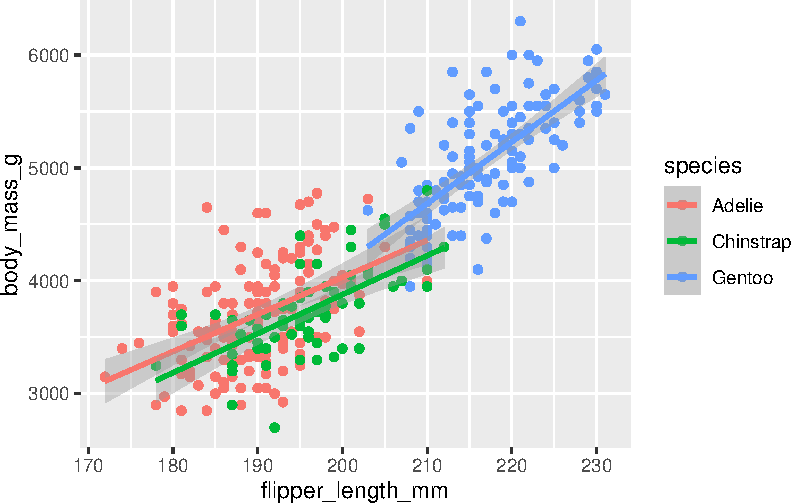
\includegraphics[keepaspectratio]{cCode_files/figure-latex/unnamed-chunk-7-1.pdf}}

\subsubsection{Python}\label{python}

\begin{tcolorbox}[enhanced jigsaw, opacityback=0, leftrule=.75mm, colback=white, left=2mm, titlerule=0mm, toprule=.15mm, toptitle=1mm, coltitle=black, title=\textcolor{quarto-callout-note-color}{\faInfo}\hspace{0.5em}{Note}, opacitybacktitle=0.6, colbacktitle=quarto-callout-note-color!10!white, breakable, bottomrule=.15mm, bottomtitle=1mm, colframe=quarto-callout-note-color-frame, arc=.35mm, rightrule=.15mm]

If the following doesn't go smoothly for you check out the additional
suggestions in the \href{python-venv.qmd}{python-venv appendix}.

\end{tcolorbox}

\paragraph{Installation}\label{installation-1}

\href{https://code.visualstudio.com/docs/languages/python}{Installation
Instructions}

Install the \texttt{mathplotlib} and \texttt{numpy} packages.

\begin{tcolorbox}[enhanced jigsaw, opacityback=0, leftrule=.75mm, colback=white, left=2mm, titlerule=0mm, toprule=.15mm, toptitle=1mm, coltitle=black, title=\textcolor{quarto-callout-tip-color}{\faLightbulb}\hspace{0.5em}{Class Discussion}, opacitybacktitle=0.6, colbacktitle=quarto-callout-tip-color!10!white, breakable, bottomrule=.15mm, bottomtitle=1mm, colframe=quarto-callout-tip-color-frame, arc=.35mm, rightrule=.15mm]

What is a ``package'' when talking about programming languages? What is
a ``library''? What is an ``executable''?

\end{tcolorbox}

\begin{tcolorbox}[enhanced jigsaw, opacityback=0, leftrule=.75mm, colback=white, left=2mm, titlerule=0mm, toprule=.15mm, toptitle=1mm, coltitle=black, title=\textcolor{quarto-callout-warning-color}{\faExclamationTriangle}\hspace{0.5em}{Warning}, opacitybacktitle=0.6, colbacktitle=quarto-callout-warning-color!10!white, breakable, bottomrule=.15mm, bottomtitle=1mm, colframe=quarto-callout-warning-color-frame, arc=.35mm, rightrule=.15mm]

Ask me about virtual environments!

\end{tcolorbox}

\href{https://dev.to/emminex/how-to-install-python-libraries-in-visual-studio-code-38i1}{setting
up a venv in vscode and python}

\paragraph{Testing}\label{testing}

\begin{tcolorbox}[enhanced jigsaw, opacityback=0, leftrule=.75mm, colback=white, left=2mm, titlerule=0mm, toprule=.15mm, toptitle=1mm, coltitle=black, title=\textcolor{quarto-callout-warning-color}{\faExclamationTriangle}\hspace{0.5em}{Warning}, opacitybacktitle=0.6, colbacktitle=quarto-callout-warning-color!10!white, breakable, bottomrule=.15mm, bottomtitle=1mm, colframe=quarto-callout-warning-color-frame, arc=.35mm, rightrule=.15mm]

You may need to install the ``reticulate'' package for R if you want to
run both python and R code in the same document as I am trying to do
here.

\end{tcolorbox}

\begin{Shaded}
\begin{Highlighting}[]
\ImportTok{import}\NormalTok{ matplotlib.pyplot }\ImportTok{as}\NormalTok{ plt}
\ImportTok{import}\NormalTok{ numpy }\ImportTok{as}\NormalTok{ np}

\CommentTok{\# fake data}
\NormalTok{np.random.seed(}\DecValTok{19680801}\NormalTok{)}
\NormalTok{data }\OperatorTok{=}\NormalTok{ np.random.lognormal(size}\OperatorTok{=}\NormalTok{(}\DecValTok{37}\NormalTok{, }\DecValTok{4}\NormalTok{), mean}\OperatorTok{=}\FloatTok{1.5}\NormalTok{, sigma}\OperatorTok{=}\FloatTok{1.75}\NormalTok{)}
\NormalTok{labels }\OperatorTok{=} \BuiltInTok{list}\NormalTok{(}\StringTok{\textquotesingle{}ABCD\textquotesingle{}}\NormalTok{)}
\NormalTok{fs }\OperatorTok{=} \DecValTok{10}  \CommentTok{\# fontsize}
\NormalTok{fig, axs }\OperatorTok{=}\NormalTok{ plt.subplots(nrows}\OperatorTok{=}\DecValTok{2}\NormalTok{, ncols}\OperatorTok{=}\DecValTok{3}\NormalTok{, figsize}\OperatorTok{=}\NormalTok{(}\DecValTok{6}\NormalTok{, }\DecValTok{6}\NormalTok{), sharey}\OperatorTok{=}\VariableTok{True}\NormalTok{)}
\NormalTok{axs[}\DecValTok{0}\NormalTok{, }\DecValTok{0}\NormalTok{].boxplot(data, tick\_labels}\OperatorTok{=}\NormalTok{labels)}
\end{Highlighting}
\end{Shaded}

\begin{verbatim}
{'whiskers': [<matplotlib.lines.Line2D object at 0x10d092e90>, <matplotlib.lines.Line2D object at 0x10d092fd0>, <matplotlib.lines.Line2D object at 0x10d093750>, <matplotlib.lines.Line2D object at 0x10d093890>, <matplotlib.lines.Line2D object at 0x10d0e4050>, <matplotlib.lines.Line2D object at 0x10d0e4190>, <matplotlib.lines.Line2D object at 0x10d0e4910>, <matplotlib.lines.Line2D object at 0x10d0e4a50>], 'caps': [<matplotlib.lines.Line2D object at 0x10d093110>, <matplotlib.lines.Line2D object at 0x10d093250>, <matplotlib.lines.Line2D object at 0x10d0939d0>, <matplotlib.lines.Line2D object at 0x10d093b10>, <matplotlib.lines.Line2D object at 0x10d0e42d0>, <matplotlib.lines.Line2D object at 0x10d0e4410>, <matplotlib.lines.Line2D object at 0x10d0e4b90>, <matplotlib.lines.Line2D object at 0x10d0e4cd0>], 'boxes': [<matplotlib.lines.Line2D object at 0x10d092d50>, <matplotlib.lines.Line2D object at 0x10d093610>, <matplotlib.lines.Line2D object at 0x10d093ed0>, <matplotlib.lines.Line2D object at 0x10d0e47d0>], 'medians': [<matplotlib.lines.Line2D object at 0x10d093390>, <matplotlib.lines.Line2D object at 0x10d093c50>, <matplotlib.lines.Line2D object at 0x10d0e4550>, <matplotlib.lines.Line2D object at 0x10d0e4e10>], 'fliers': [<matplotlib.lines.Line2D object at 0x10d0934d0>, <matplotlib.lines.Line2D object at 0x10d093d90>, <matplotlib.lines.Line2D object at 0x10d0e4690>, <matplotlib.lines.Line2D object at 0x10d0e4f50>], 'means': []}
\end{verbatim}

\begin{Shaded}
\begin{Highlighting}[]
\NormalTok{axs[}\DecValTok{0}\NormalTok{, }\DecValTok{0}\NormalTok{].set\_title(}\StringTok{\textquotesingle{}Default\textquotesingle{}}\NormalTok{, fontsize}\OperatorTok{=}\NormalTok{fs)}

\NormalTok{axs[}\DecValTok{0}\NormalTok{, }\DecValTok{1}\NormalTok{].boxplot(data, tick\_labels}\OperatorTok{=}\NormalTok{labels, showmeans}\OperatorTok{=}\VariableTok{True}\NormalTok{)}
\end{Highlighting}
\end{Shaded}

\begin{verbatim}
{'whiskers': [<matplotlib.lines.Line2D object at 0x10d0e51d0>, <matplotlib.lines.Line2D object at 0x10d0e5310>, <matplotlib.lines.Line2D object at 0x10d0e5bd0>, <matplotlib.lines.Line2D object at 0x10d0e5d10>, <matplotlib.lines.Line2D object at 0x10d0e65d0>, <matplotlib.lines.Line2D object at 0x10d0e6710>, <matplotlib.lines.Line2D object at 0x10d0e6fd0>, <matplotlib.lines.Line2D object at 0x10d0e7110>], 'caps': [<matplotlib.lines.Line2D object at 0x10d0e5450>, <matplotlib.lines.Line2D object at 0x10d0e5590>, <matplotlib.lines.Line2D object at 0x10d0e5e50>, <matplotlib.lines.Line2D object at 0x10d0e5f90>, <matplotlib.lines.Line2D object at 0x10d0e6850>, <matplotlib.lines.Line2D object at 0x10d0e6990>, <matplotlib.lines.Line2D object at 0x10d0e7250>, <matplotlib.lines.Line2D object at 0x10d0e7390>], 'boxes': [<matplotlib.lines.Line2D object at 0x10d0e5090>, <matplotlib.lines.Line2D object at 0x10d0e5a90>, <matplotlib.lines.Line2D object at 0x10d0e6490>, <matplotlib.lines.Line2D object at 0x10d0e6e90>], 'medians': [<matplotlib.lines.Line2D object at 0x10d0e56d0>, <matplotlib.lines.Line2D object at 0x10d0e60d0>, <matplotlib.lines.Line2D object at 0x10d0e6ad0>, <matplotlib.lines.Line2D object at 0x10d0e74d0>], 'fliers': [<matplotlib.lines.Line2D object at 0x10d0e5950>, <matplotlib.lines.Line2D object at 0x10d0e6350>, <matplotlib.lines.Line2D object at 0x10d0e6d50>, <matplotlib.lines.Line2D object at 0x10d0e7750>], 'means': [<matplotlib.lines.Line2D object at 0x10d0e5810>, <matplotlib.lines.Line2D object at 0x10d0e6210>, <matplotlib.lines.Line2D object at 0x10d0e6c10>, <matplotlib.lines.Line2D object at 0x10d0e7610>]}
\end{verbatim}

\begin{Shaded}
\begin{Highlighting}[]
\NormalTok{axs[}\DecValTok{0}\NormalTok{, }\DecValTok{1}\NormalTok{].set\_title(}\StringTok{\textquotesingle{}showmeans=True\textquotesingle{}}\NormalTok{, fontsize}\OperatorTok{=}\NormalTok{fs)}

\NormalTok{axs[}\DecValTok{0}\NormalTok{, }\DecValTok{2}\NormalTok{].boxplot(data, tick\_labels}\OperatorTok{=}\NormalTok{labels, showmeans}\OperatorTok{=}\VariableTok{True}\NormalTok{, meanline}\OperatorTok{=}\VariableTok{True}\NormalTok{)}
\end{Highlighting}
\end{Shaded}

\begin{verbatim}
{'whiskers': [<matplotlib.lines.Line2D object at 0x10d0e79d0>, <matplotlib.lines.Line2D object at 0x10d0e7b10>, <matplotlib.lines.Line2D object at 0x10d154410>, <matplotlib.lines.Line2D object at 0x10d154550>, <matplotlib.lines.Line2D object at 0x10d154e10>, <matplotlib.lines.Line2D object at 0x10d154f50>, <matplotlib.lines.Line2D object at 0x10d155810>, <matplotlib.lines.Line2D object at 0x10d155950>], 'caps': [<matplotlib.lines.Line2D object at 0x10d0e7c50>, <matplotlib.lines.Line2D object at 0x10d0e7d90>, <matplotlib.lines.Line2D object at 0x10d154690>, <matplotlib.lines.Line2D object at 0x10d1547d0>, <matplotlib.lines.Line2D object at 0x10d155090>, <matplotlib.lines.Line2D object at 0x10d1551d0>, <matplotlib.lines.Line2D object at 0x10d155a90>, <matplotlib.lines.Line2D object at 0x10d155bd0>], 'boxes': [<matplotlib.lines.Line2D object at 0x10cbd7b10>, <matplotlib.lines.Line2D object at 0x10d1542d0>, <matplotlib.lines.Line2D object at 0x10d154cd0>, <matplotlib.lines.Line2D object at 0x10d1556d0>], 'medians': [<matplotlib.lines.Line2D object at 0x10d0e7ed0>, <matplotlib.lines.Line2D object at 0x10d154910>, <matplotlib.lines.Line2D object at 0x10d155310>, <matplotlib.lines.Line2D object at 0x10d155d10>], 'fliers': [<matplotlib.lines.Line2D object at 0x10d154190>, <matplotlib.lines.Line2D object at 0x10d154b90>, <matplotlib.lines.Line2D object at 0x10d155590>, <matplotlib.lines.Line2D object at 0x10d155f90>], 'means': [<matplotlib.lines.Line2D object at 0x10d154050>, <matplotlib.lines.Line2D object at 0x10d154a50>, <matplotlib.lines.Line2D object at 0x10d155450>, <matplotlib.lines.Line2D object at 0x10d155e50>]}
\end{verbatim}

\begin{Shaded}
\begin{Highlighting}[]
\NormalTok{axs[}\DecValTok{0}\NormalTok{, }\DecValTok{2}\NormalTok{].set\_title(}\StringTok{\textquotesingle{}showmeans=True,}\CharTok{\textbackslash{}n}\StringTok{meanline=True\textquotesingle{}}\NormalTok{, fontsize}\OperatorTok{=}\NormalTok{fs)}

\NormalTok{axs[}\DecValTok{1}\NormalTok{, }\DecValTok{0}\NormalTok{].boxplot(data, tick\_labels}\OperatorTok{=}\NormalTok{labels, showbox}\OperatorTok{=}\VariableTok{False}\NormalTok{, showcaps}\OperatorTok{=}\VariableTok{False}\NormalTok{)}
\end{Highlighting}
\end{Shaded}

\begin{verbatim}
{'whiskers': [<matplotlib.lines.Line2D object at 0x10d156350>, <matplotlib.lines.Line2D object at 0x10d156490>, <matplotlib.lines.Line2D object at 0x10d156850>, <matplotlib.lines.Line2D object at 0x10d156990>, <matplotlib.lines.Line2D object at 0x10d156d50>, <matplotlib.lines.Line2D object at 0x10d156e90>, <matplotlib.lines.Line2D object at 0x10d157250>, <matplotlib.lines.Line2D object at 0x10d157390>], 'caps': [], 'boxes': [], 'medians': [<matplotlib.lines.Line2D object at 0x10d1565d0>, <matplotlib.lines.Line2D object at 0x10d156ad0>, <matplotlib.lines.Line2D object at 0x10d156fd0>, <matplotlib.lines.Line2D object at 0x10d1574d0>], 'fliers': [<matplotlib.lines.Line2D object at 0x10d156710>, <matplotlib.lines.Line2D object at 0x10d156c10>, <matplotlib.lines.Line2D object at 0x10d157110>, <matplotlib.lines.Line2D object at 0x10d157610>], 'means': []}
\end{verbatim}

\begin{Shaded}
\begin{Highlighting}[]
\NormalTok{tufte\_title }\OperatorTok{=} \StringTok{\textquotesingle{}Tufte Style }\CharTok{\textbackslash{}n}\StringTok{(showbox=False,}\CharTok{\textbackslash{}n}\StringTok{showcaps=False)\textquotesingle{}}
\NormalTok{axs[}\DecValTok{1}\NormalTok{, }\DecValTok{0}\NormalTok{].set\_title(tufte\_title, fontsize}\OperatorTok{=}\NormalTok{fs)}

\NormalTok{axs[}\DecValTok{1}\NormalTok{, }\DecValTok{1}\NormalTok{].boxplot(data, tick\_labels}\OperatorTok{=}\NormalTok{labels, notch}\OperatorTok{=}\VariableTok{True}\NormalTok{, bootstrap}\OperatorTok{=}\DecValTok{10000}\NormalTok{)}
\end{Highlighting}
\end{Shaded}

\begin{verbatim}
{'whiskers': [<matplotlib.lines.Line2D object at 0x10d157890>, <matplotlib.lines.Line2D object at 0x10d1579d0>, <matplotlib.lines.Line2D object at 0x10d1d0190>, <matplotlib.lines.Line2D object at 0x10d1d02d0>, <matplotlib.lines.Line2D object at 0x10d1d0a50>, <matplotlib.lines.Line2D object at 0x10d1d0b90>, <matplotlib.lines.Line2D object at 0x10d1d1310>, <matplotlib.lines.Line2D object at 0x10d1d1450>], 'caps': [<matplotlib.lines.Line2D object at 0x10d157b10>, <matplotlib.lines.Line2D object at 0x10d157c50>, <matplotlib.lines.Line2D object at 0x10d1d0410>, <matplotlib.lines.Line2D object at 0x10d1d0550>, <matplotlib.lines.Line2D object at 0x10d1d0cd0>, <matplotlib.lines.Line2D object at 0x10d1d0e10>, <matplotlib.lines.Line2D object at 0x10d1d1590>, <matplotlib.lines.Line2D object at 0x10d1d16d0>], 'boxes': [<matplotlib.lines.Line2D object at 0x10d157750>, <matplotlib.lines.Line2D object at 0x10d1d0050>, <matplotlib.lines.Line2D object at 0x10d1d0910>, <matplotlib.lines.Line2D object at 0x10d1d11d0>], 'medians': [<matplotlib.lines.Line2D object at 0x10d157d90>, <matplotlib.lines.Line2D object at 0x10d1d0690>, <matplotlib.lines.Line2D object at 0x10d1d0f50>, <matplotlib.lines.Line2D object at 0x10d1d1810>], 'fliers': [<matplotlib.lines.Line2D object at 0x10d157ed0>, <matplotlib.lines.Line2D object at 0x10d1d07d0>, <matplotlib.lines.Line2D object at 0x10d1d1090>, <matplotlib.lines.Line2D object at 0x10d1d1950>], 'means': []}
\end{verbatim}

\begin{Shaded}
\begin{Highlighting}[]
\NormalTok{axs[}\DecValTok{1}\NormalTok{, }\DecValTok{1}\NormalTok{].set\_title(}\StringTok{\textquotesingle{}notch=True,}\CharTok{\textbackslash{}n}\StringTok{bootstrap=10000\textquotesingle{}}\NormalTok{, fontsize}\OperatorTok{=}\NormalTok{fs)}

\NormalTok{axs[}\DecValTok{1}\NormalTok{, }\DecValTok{2}\NormalTok{].boxplot(data, tick\_labels}\OperatorTok{=}\NormalTok{labels, showfliers}\OperatorTok{=}\VariableTok{False}\NormalTok{)}
\end{Highlighting}
\end{Shaded}

\begin{verbatim}
{'whiskers': [<matplotlib.lines.Line2D object at 0x10d1d1bd0>, <matplotlib.lines.Line2D object at 0x10d1d1d10>, <matplotlib.lines.Line2D object at 0x10d1d2350>, <matplotlib.lines.Line2D object at 0x10d1d2490>, <matplotlib.lines.Line2D object at 0x10d1d2ad0>, <matplotlib.lines.Line2D object at 0x10d1d2c10>, <matplotlib.lines.Line2D object at 0x10d1d3250>, <matplotlib.lines.Line2D object at 0x10d1d3390>], 'caps': [<matplotlib.lines.Line2D object at 0x10d1d1e50>, <matplotlib.lines.Line2D object at 0x10d1d1f90>, <matplotlib.lines.Line2D object at 0x10d1d25d0>, <matplotlib.lines.Line2D object at 0x10d1d2710>, <matplotlib.lines.Line2D object at 0x10d1d2d50>, <matplotlib.lines.Line2D object at 0x10d1d2e90>, <matplotlib.lines.Line2D object at 0x10d1d34d0>, <matplotlib.lines.Line2D object at 0x10d1d3610>], 'boxes': [<matplotlib.lines.Line2D object at 0x10d1d1a90>, <matplotlib.lines.Line2D object at 0x10d1d2210>, <matplotlib.lines.Line2D object at 0x10d1d2990>, <matplotlib.lines.Line2D object at 0x10d1d3110>], 'medians': [<matplotlib.lines.Line2D object at 0x10d1d20d0>, <matplotlib.lines.Line2D object at 0x10d1d2850>, <matplotlib.lines.Line2D object at 0x10d1d2fd0>, <matplotlib.lines.Line2D object at 0x10d1d3750>], 'fliers': [], 'means': []}
\end{verbatim}

\begin{Shaded}
\begin{Highlighting}[]
\NormalTok{axs[}\DecValTok{1}\NormalTok{, }\DecValTok{2}\NormalTok{].set\_title(}\StringTok{\textquotesingle{}showfliers=False\textquotesingle{}}\NormalTok{, fontsize}\OperatorTok{=}\NormalTok{fs)}

\ControlFlowTok{for}\NormalTok{ ax }\KeywordTok{in}\NormalTok{ axs.flat:}
\NormalTok{    ax.set\_yscale(}\StringTok{\textquotesingle{}log\textquotesingle{}}\NormalTok{)}
\NormalTok{    ax.set\_yticklabels([])}
\end{Highlighting}
\end{Shaded}

\begin{verbatim}
[Text(0, 0.001, ''), Text(0, 0.01, ''), Text(0, 0.1, ''), Text(0, 1.0, ''), Text(0, 10.0, ''), Text(0, 100.0, ''), Text(0, 1000.0, ''), Text(0, 10000.0, '')]
[]
[]
[Text(0, 0.001, ''), Text(0, 0.01, ''), Text(0, 0.1, ''), Text(0, 1.0, ''), Text(0, 10.0, ''), Text(0, 100.0, ''), Text(0, 1000.0, ''), Text(0, 10000.0, '')]
[]
[]
\end{verbatim}

\begin{Shaded}
\begin{Highlighting}[]

\NormalTok{fig.subplots\_adjust(hspace}\OperatorTok{=}\FloatTok{0.4}\NormalTok{)}
\end{Highlighting}
\end{Shaded}

\pandocbounded{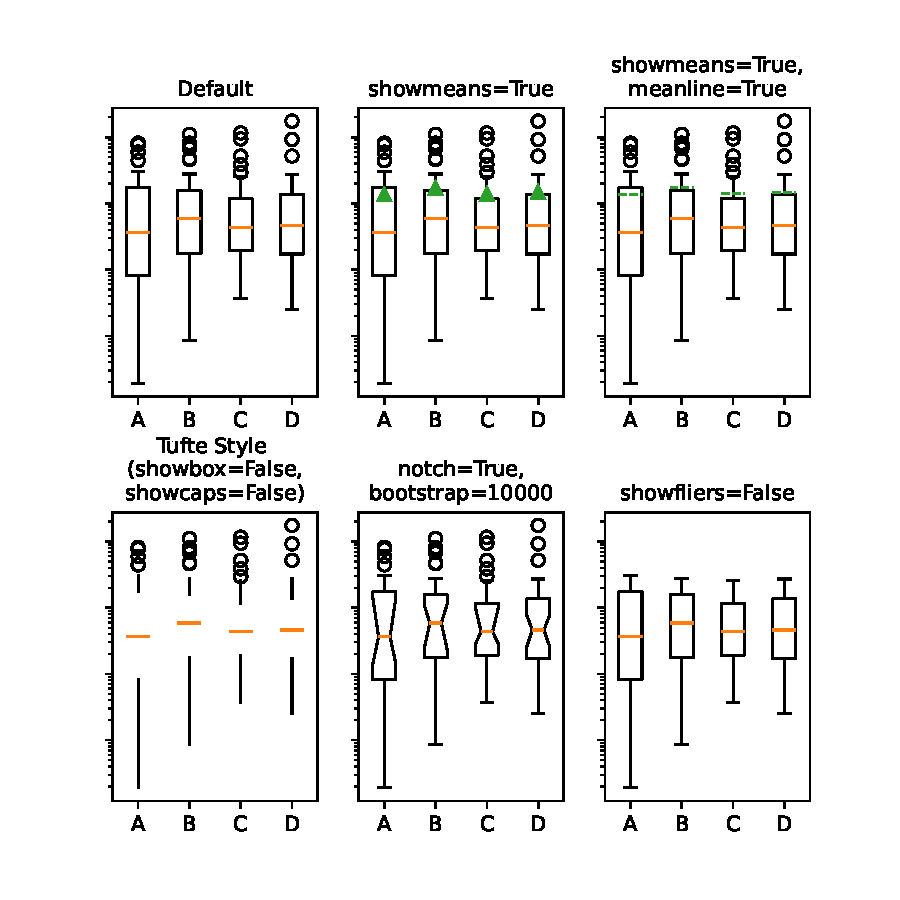
\includegraphics[keepaspectratio]{cCode_files/figure-latex/unnamed-chunk-8-1.pdf}}

\subsubsection{Javascript}\label{javascript}

\bookmarksetup{startatroot}

\chapter{Writing Scientific
Documents}\label{writing-scientific-documents}

Papers Posters Websites Books Math Formulas Images Graphs References
Analyses/Code

What is RStudio? What happened to RStudio? How does Quarto relate to
RStudio? What languages does it support? Can you write code in it? Can
you write text in it? Can you write an article in it?

\subsection{Scientific Publishing
Tools}\label{scientific-publishing-tools}

What is a markup language?

What are the advantages/disadvantages of using a tool other that Word
for writing up your research?

Write once use everywhere.

Some of the available options.

\begin{itemize}
\tightlist
\item
  \href{https://www.latex-project.org/}{LaTeX} This was the standard for
  several decades, and used more by mathematicians than others, but
  today it seems limited in that it produces mostly pdfs, and many
  people also want their files to export to html (webpages)
\item
  \href{https://ctan.math.washington.edu/tex-archive/info/latex4wp/latex4wp.pdf}{A
  guide to LaTex for Word Users (pdf)}
\item
  The descendants of
  \href{https://en.wikipedia.org/wiki/Markdown}{markdown}
\item
  \href{https://quarto.org/}{Quarto} (we will skip Rmd and since we are
  using its successor qmd. Both are related to the people who wrote
  RStudio,\texttt{knitr}, and are now known as
  \href{https://posit.co/}{Posit}).
\end{itemize}

Here are some of the helper links for things we can do with Quarto: -
\href{https://quarto.org/docs/journals/}{journal formats} try the
Elsevier format for this course. A lot of psych journals are Elsevier
owned. -
\href{https://jjallaire.quarto.pub/reproducible-manuscripts-with-quarto/\#/title-slide}{presentation}
-
\href{https://danielroelfs.com/blog/sql-notebooks-with-quarto/}{Talking
to databases}. -
\href{https://beamilz.com/posts/2022-06-05-creating-a-blog-with-quarto/en/}{Make
a website/blog for your work or lab} -
\href{https://github.com/mcanouil/awesome-quarto?tab=readme-ov-file}{And
more \ldots{}}

\bookmarksetup{startatroot}

\chapter{In Lab Experiments}\label{in-lab-experiments}

\begin{itemize}
\tightlist
\item
  Making stuff appear on monitors.
\item
  What is OpenGL?
\item
  Use pygame to make some simple visual experiments.
\item
  Have a beauty contest the following week to see what people have been
  able to make?
\item
  Make sure that people are using
  \href{https://python.land/virtual-environments/virtualenv}{venv}
\end{itemize}

\subsection{Online Experiments}\label{online-experiments}

Running a server for testing and more?
\href{https://www.apachefriends.org/index.html}{XAMPP} Running a lab now
seems to require some familiarity with servers. And people who want to
write their experiments in javascript often want to try things out first
so it seems something like
\href{https://www.apachefriends.org/download.html}{XAMPP} might be a
good resource. \emph{Exercise} to download and get the XAMPP server
running? Need to expand this. An exercise with
\href{https://code.visualstudio.com/Docs/languages/javascript}{JavaScript}?
This
\href{https://www.geeksforgeeks.org/how-to-display-images-in-javascript/}{site}
has a simple bit of code for throwing an image on the screen. Then use
the XAMPP server to test it? Require changing the image? Animate a
button to toggle or get a random image?

\bookmarksetup{startatroot}

\chapter{What are some of the challenges that computational tools pose
for
reproducibility?}\label{what-are-some-of-the-challenges-that-computational-tools-pose-for-reproducibility}

\begin{tcolorbox}[enhanced jigsaw, opacityback=0, leftrule=.75mm, colback=white, left=2mm, titlerule=0mm, toprule=.15mm, toptitle=1mm, coltitle=black, title=\textcolor{quarto-callout-tip-color}{\faLightbulb}\hspace{0.5em}{Classroom Exercise}, opacitybacktitle=0.6, colbacktitle=quarto-callout-tip-color!10!white, breakable, bottomrule=.15mm, bottomtitle=1mm, colframe=quarto-callout-tip-color-frame, arc=.35mm, rightrule=.15mm]

Read and discuss:
\href{https://www.nature.com/articles/d41586-018-05990-5}{A toolkit for
transparency \ldots{}}.

\end{tcolorbox}

\bookmarksetup{startatroot}

\chapter{\texorpdfstring{Knowledge Management
(\href{https://en.wikipedia.org/wiki/Zettelkasten}{Zettlekasten})}{Knowledge Management (Zettlekasten)}}\label{knowledge-management-zettlekasten}

\begin{enumerate}
\def\labelenumi{\arabic{enumi}.}
\tightlist
\item
  \href{https://github.com/org-roam/org-roam}{Org-roam}
\item
  \href{https://github.com/dendronhq/dendron}{Dendron} - works with VS
  Code
\item
  \href{https://obsidian.md/}{Obsidian}
\end{enumerate}

\bookmarksetup{startatroot}

\chapter{Reference Management}\label{reference-management}

\begin{itemize}
\tightlist
\item
  What is \href{https://www.crossref.org/}{Crossref}?
\item
  What is a \href{https://www.doi.org/}{doi}?
\item
  What is an \href{https://orcid.org/}{orcid}?
\item
  What is \href{https://www.zotero.org/}{zotero}?
\item
  What is \href{https://citationstyles.org/}{csl}?
\end{itemize}

\begin{tcolorbox}[enhanced jigsaw, opacityback=0, leftrule=.75mm, colback=white, left=2mm, titlerule=0mm, toprule=.15mm, toptitle=1mm, coltitle=black, title=\textcolor{quarto-callout-tip-color}{\faLightbulb}\hspace{0.5em}{Classroom Exercise}, opacitybacktitle=0.6, colbacktitle=quarto-callout-tip-color!10!white, breakable, bottomrule=.15mm, bottomtitle=1mm, colframe=quarto-callout-tip-color-frame, arc=.35mm, rightrule=.15mm]

Locate and download the csl file for the current APA style and also for
one at least one other non-apa style.

\end{tcolorbox}

\section{Using References With Quatro and VS
Code}\label{using-references-with-quatro-and-vs-code}

\section{Using References With
Overleaf}\label{using-references-with-overleaf}

VS Code is not your only option. Overleaf also use ``.bib'' files to
hold references, though some of the other syntax is different.

Here are some links to get you started with references in overleaf. 1.
\href{https://www.overleaf.com/learn/how-to/How_to_link_your_Overleaf_account_to_Mendeley_and_Zotero}{Linking
Overleaf and Zotero} 2. {[}Connecting Zotero and
Quarto{]}(https://quarto.org/docs/visual-editor/technical.html\#citations-from-zotero)

\section{Poster Presentations ? (MOVE THIS
SECTION)}\label{poster-presentations-move-this-section}

{[}Scientific Posters with
Quarto{]}(https://github.com/quarto-ext/typst-templates/tree/main/poster)

\href{https://www.overleaf.com/learn/latex/Knitr}{LaTeX and Knitr in
Overleaf}{]}{[}knitr{]}{]} with overleaf.
\href{https://www.overleaf.com/latex/templates?q=poster}{A scientific
poster with Overleaf?}

\bookmarksetup{startatroot}

\chapter{Finding Citations}\label{finding-citations}

\begin{itemize}
\tightlist
\item
  \href{https://www.semanticscholar.org/}{Semantic Scholar}
\item
  \href{https://openalex.org/}{OpenAlex}
\item
  \href{https://scholar.google.ca/}{Google Scholar}
\item
  \href{https://consensus.app/}{Consensus}
\item
  \href{https://www.undermind.ai/home/}{Undermind}
\end{itemize}

\bookmarksetup{startatroot}

\chapter{Testing Your Javascript}\label{testing-your-javascript}

\section{Run your own server locally}\label{run-your-own-server-locally}

Running a lab now seems to require some familiarity with servers. And
people who want to write their experiments in javascript often want to
try things out first so it seems something like XAMMP is a good tool to
know about.

\subsection{XAMPP}\label{xampp}

\href{https://www.apachefriends.org/index.html}{XAMMP}

\subsubsection{Downloading}\label{downloading}

\href{https://www.apachefriends.org/download.html}{Download link}

\subsection{In Lab Experiments}\label{in-lab-experiments-1}

\begin{itemize}
\tightlist
\item
  Making stuff appear on monitors.
\item
  What is OpenGL?
\item
  Use pygame to make some simple visual experiments.
\item
  Have a beauty contest the following week to see what people have been
  able to make?
\item
  Make sure that people are using
  \href{https://python.land/virtual-environments/virtualenv}{venv}
\end{itemize}

\subsection{Online Experiments}\label{online-experiments-1}

An exercise with
\href{https://code.visualstudio.com/Docs/languages/javascript}{JavaScript}?
This
\href{https://www.geeksforgeeks.org/how-to-display-images-in-javascript/}{site}
has a simple bit of code for throwing an image on the screen.

Can you use the XAMPP server to test it? Require changing the image?
Animate a button to toggle or get a random image? WIP HERE

\bookmarksetup{startatroot}

\chapter{Large Language Models}\label{large-language-models}

\section{Run locally}\label{run-locally}

Why? Own your own data.

Security and Privacy.

Research applications you may not want participants' data fed to openAI
or other proprietary vendors.

\section{How to?}\label{how-to}

There are many methods to running LLMs locally on your own hardward. I
have chosen \href{https://www.nomic.ai/gpt4all}{GPT4All}. It can run
under OSX, Windows, and Ubuntu (linux).

\subsection{Key Features of GPT4ALL}\label{key-features-of-gpt4all}

According to the website
https://getstream.io/blog/best-local-llm-tools/:

GPT4All can run LLMs on major consumer hardware such as Mac M-Series
chips, AMD and NVIDIA GPUs. The following are its key features.

\begin{itemize}
\item
  Privacy First: Keep private and sensitive chat information and prompts
  only on your machine.
\item
  No Internet Required: It works completely offline.
\item
  Models Exploration: This feature allows developers to browse and
  download different kinds of LLMs to experiment with. You can select
  about 1000 open-source language models from popular options like
  LLama, Mistral, and more.
\item
  Local Documents: You can let your local LLM access your sensitive data
  with local documents like .pdf and .txt without data leaving your
  device and without a network.
\item
  Customization options: It provides several chatbot adjustment options
  like temperature, batch size, context length, etc.
\item
  Enterprise Edition: GPT4ALL provides an enterprise package with
  security, support, and per-device licenses to bring local AI to
  businesses.
\end{itemize}

It is also a very popular LLM for self-hosting (second only to Ollama,
which you should also try out).

\section{How-to}\label{how-to-1}

From the GPT4all download page download the version for your operating
system.

Follow the download instructions appropriate to your system and pay
particular attention to any warnings and make sure that you have
sufficient freespace. This is a big application and the model parameters
are also quite large.

After you have successfully downloaded and installed the program
checkout the
\href{https://docs.gpt4all.io/gpt4all_desktop/quickstart.html}{quickstart
guide}.

\begin{enumerate}
\def\labelenumi{\arabic{enumi}.}
\tightlist
\item
  Start Chatting
\item
  Install a Model
\item
  I tried ``Llama 3.2 1b Instruct''
\item
  Load the model
\item
  Start chatting
\end{enumerate}

\section{Using LLMs for Dynamic
Research}\label{using-llms-for-dynamic-research}

What are the mechanics we need for this? We need our model to accept
input and generate output and we need a method to transfer the elements
of the conversation back and forth. The first stage is to think of the
components we have used so far and how we might stitch them together for
this task.

It is also a useful transitional step to work incrementally. First,
maybe try to set up an interface to allow someone to talk to the model
via a web interface. Then you might be able to figure out how to use
\href{link}{GET and POST} from PHP to communicate between two web
servers. There are definitely better ways to do that, but it is a fairly
direct starting point. If you want an additional challenge perhaps try
to use the tool:
\href{https://medium.com/@kevinkoech265/curl-a-deep-dive-into-command-line-data-transfer-8361a85b177d}{curl}.

\begin{tcolorbox}[enhanced jigsaw, opacityback=0, leftrule=.75mm, colback=white, left=2mm, titlerule=0mm, toprule=.15mm, toptitle=1mm, coltitle=black, title=\textcolor{quarto-callout-tip-color}{\faLightbulb}\hspace{0.5em}{Classroom Exercise}, opacitybacktitle=0.6, colbacktitle=quarto-callout-tip-color!10!white, breakable, bottomrule=.15mm, bottomtitle=1mm, colframe=quarto-callout-tip-color-frame, arc=.35mm, rightrule=.15mm]

Download and implement the above.

Start the GPT4All Server

See if you can get your GPT4All model to talk to another group's model.

\end{tcolorbox}

\section{Why Might You Want To Do
This?}\label{why-might-you-want-to-do-this}

\href{https://www.science.org/doi/10.1126/science.adq1814}{Durably
reducing conspiracy beliefs through dialogues with AI}

\url{https://www.youtube.com/watch?v=qD1fnYDTbHM}

\href{https://www.linkedin.com/pulse/integrate-chatgpt-openai-api-your-research-project-part-ding-wang-rdyec}{This}
LinkedIn post talks about ChatGPT integration. What would you have to
change to get it working with your local server?

\begin{tcolorbox}[enhanced jigsaw, opacityback=0, leftrule=.75mm, colback=white, left=2mm, titlerule=0mm, toprule=.15mm, toptitle=1mm, coltitle=black, title=\textcolor{quarto-callout-tip-color}{\faLightbulb}\hspace{0.5em}{Class Question}, opacitybacktitle=0.6, colbacktitle=quarto-callout-tip-color!10!white, breakable, bottomrule=.15mm, bottomtitle=1mm, colframe=quarto-callout-tip-color-frame, arc=.35mm, rightrule=.15mm]

What is a RAG in this context?

\end{tcolorbox}

\section{Next steps}\label{next-steps}

Recently (Duan, Li, and Cai 2024) has published an R package to make all
of this easier. The
\href{https://github.com/xufengduan/MacBehaviour}{github repository} has
the library, a ``read-me'' and installation instructions. Our
\emph{class activity} is to see if anyone can get this up and working by
next week.

\bookmarksetup{startatroot}

\chapter{Databases and management}\label{databases-and-management}

\begin{itemize}
\tightlist
\item
  \href{https://www.dataversity.net/what-is-database-management/}{What
  is it}
\item
  \href{https://learning-oreilly-com.proxy.lib.uwaterloo.ca/library/view/getting-started-with/9781803241005/B18270_01.xhtml\#_idTextAnchor015}{A
  book on DuckDB - database stuff}
\item
  \href{https://mariadb.org/}{MariaDB} This SQL like, and open source.
  Might be easier to get started with and still be SQL enough to give
  them some professional benefits. I was thinking we could get some data
  online, often they come as CSV's and read it into the database? This
  is \href{https://www.simplified.guide/mysql-mariadb/import-csv}{one
  example} how. A
  \href{https://kinsta.com/blog/mariadb-vs-postgresql/}{blog} that
  compares MariaDB to SQL. A
  \href{https://mariadb.com/kb/en/mariadb-basics/}{quickie tutorial}.
\item
  Why would I want to use a relational database over a csv file (or R
  data frame or similar)? This could be a class exercise and discussion.
\item
  \emph{Exercise} Download MariaDB
\end{itemize}

\subsection{Datascience}\label{datascience}

\begin{itemize}
\tightlist
\item
  \href{https://medium.com/@fareedkhandev/complete-roadmap-of-data-science-for-non-cs-cs-students-equivalent-to-a-degree-1a0a810360c0}{one
  person's roadmap for non-cs grads}
\end{itemize}

\subsection{Grant Funding}\label{grant-funding}

At the moment I am not sure if will have time for this. But thinking of
having the students review the peer review manual for NSERC Discovery
Grants. Then have them each write a minimal proposal. Assign the
proposals to members of the class, and then hold our own reviewers
meeting to decide which projects to fund. Top grants get performed for
experiments? Get extra-credit points?

\bookmarksetup{startatroot}

\chapter{Summary}\label{summary}

In summary, I have not gotten to writing a summary yet.

\cleardoublepage
\phantomsection
\addcontentsline{toc}{part}{Appendices}
\appendix

\chapter{Version Control}\label{sec-versionControl}

\section{Getting Started - Some old videos on git from
PSYCH363/310}\label{getting-started---some-old-videos-on-git-from-psych363310}

A few years ago when I was teaching a more elementary version of some of
this material (PSYCH363) I included some videos on git and using Github.
Some components of these videos may be a bit out of date, and a few
things about the interface have changed. Still they may be a reasonable
starting point for those of you who feel you need a refresher on version
control. Note that for PSYCH390 I am assuming you can either already use
version control or figure it out on your own. I will give some class
time for getting things working, but mostly you will have to pursue this
on your own. The notes here are intended to be prompts and guides, but
not to be comprehensive.

You will notice that in the videos I talk a lot about Linux. We are not
using that for this course so you can ignore those references. However,
I do demonstrate the use in the \emph{terminal}. That is available to
all of you regardless of operating system. You will just have to find
your own OS version of it.

Frequenly you will see this referred to as a command line tool
(``cli''). It is now easier to get \href{https://cli.github.com/}{this}
this working on Windows and OSX than it used to be. For OSX you can also
check out \textbf{Homebrew}. For the adventurous Windows user you can
look at WSL2.

\section{An overview of git and
Github}\label{an-overview-of-git-and-github}

\url{https://vimeo.com/456349738}

\section{You have choices - other version control
system}\label{you-have-choices---other-version-control-system}

\begin{enumerate}
\def\labelenumi{\arabic{enumi}.}
\tightlist
\item
  \href{https://www.mercurial-scm.org/}{Mercurial}
\item
  \href{http://darcs.net/}{Darcs}
\item
  \href{https://www.nongnu.org/cvs/}{CVS}
\item
  \href{https://subversion.apache.org/}{Subversion}
\item
  \href{https://pijul.org/}{Pijul}
\end{enumerate}

Each has their own fans. CVS and Subversion are more legacy options, but
you will still see them occasionally. Darcs is more of an experiment
than a broadly used system. Mercurial used to be the cool kid, but now
seems eclipsed by \emph{Pijul}. That is the one for experimental users.

\section{Git is not Github}\label{git-is-not-github}

Git is the version control software. Github is a very popular place to
host your publically accessible git repository, but it is far from your
only option. You can host elsewhere.

\begin{enumerate}
\def\labelenumi{\arabic{enumi}.}
\tightlist
\item
  \href{https://osf.io/}{OSF.io} For scientists OSF.io seeks to make
  itself a way to host scientific projects and their data. Trivia
  question? Do I have any repositories on Osf.io?
\item
  \href{https://sourceforge.net/}{Sourceforge} An oldie, but still used.
\item
  \href{https://bitbucket.org/}{Bitbucket}
\item
  Gitlab The university provides you with a gitlab account:
  \url{https://git.uwaterloo.ca}
\item
  \href{https://codeberg.org/}{Codeberg} If you believe in freedom and
  neck beards.
\end{enumerate}

\section{Things you should do}\label{things-you-should-do}

\begin{enumerate}
\def\labelenumi{\arabic{enumi}.}
\tightlist
\item
  Install git
\item
  Get an account on github
\item
  Fork the course repository
\item
  Clone the course repository to your laptop
\item
  Set up my version as an additional \textbf{remote}.
\item
  See if you can make a ``pull request'' to me. You may find that you
  have to set up an \textbf{ssh key} in order to efficiently pull and
  push to Github. Github has very clear
  \href{https://docs.github.com/en/authentication/connecting-to-github-with-ssh/generating-a-new-ssh-key-and-adding-it-to-the-ssh-agent}{instructions}
  on how to go about doing this.
\end{enumerate}

\section{But first}\label{but-first}

If you have not used git before you will have to configure git. It needs
to know who you are and how to reach you at least.

You can execute commands like this in your terminal:

\begin{Shaded}
\begin{Highlighting}[]
\FunctionTok{git}\NormalTok{ config }\AttributeTok{{-}{-}global}\NormalTok{ user.name }\StringTok{"John Doe"}
\FunctionTok{git}\NormalTok{ config }\AttributeTok{{-}{-}global}\NormalTok{ user.email johndoe@example.com}
\end{Highlighting}
\end{Shaded}

More on these configuration options can be found
\href{https://git-scm.com/book/en/v2/Getting-Started-First-Time-Git-Setup}{in
a nice online book}.

\section{Understanding Git and the Workflow in
Pictures}\label{understanding-git-and-the-workflow-in-pictures}

When starting to use git I found it very confusing to tell what was
where and what direction things were going when I pushed and pulled. I
found pictures helpful adjuncts to the prose descriptions. A few helpful
illustrations to the distinction of clones, forks, pull, push, and pull
request can be found
\href{https://www.toolsqa.com/git/difference-between-git-clone-and-git-fork/}{here}.

I also made a little video to try and illustrate some of these concepts
a few years ago. Read for the gist and not for the specific examples.

\url{https://vimeo.com/456349595}

\section{Principal Terms to Learn
First}\label{principal-terms-to-learn-first}

\begin{itemize}
\tightlist
\item
  \textbf{Fork:} A copy of one github repository to another
  \textbf{github} repository.
\item
  \textbf{Clone:} A copy of one \textbf{git} repository to another
  \textbf{git} repository. The first repository might be hosted on
  github, but the second one, the \emph{cloned} one exists on a local
  machine. In your case this is probably your laptop.
\item
  \textbf{Remote:} This is a repository that you are following. You will
  typically \emph{pull} from these, but your \emph{push} permissions may
  be limited depending on the distinctions between forks and clones, and
  whether you own the remote or someone else does. You can have more
  than one remote.
\item
  \textbf{Pull:} the transfer of information and changes \textbf{from}
  one repository incorporated into another. This is how you get the new
  information from a remote transported to a local repository that you
  control.
\item
  \textbf{Push:} this is the transfer of information \textbf{to} a
  repository you control (or have permissions to push to) from another
  repository that you control. This is often from your local laptop
  version to the hosted repository (your fork) on github.
\item
  \textbf{Pull Request:} When you have information or changes that you
  think would be helpful to a remote you do \textbf{not} have push
  permissions for then you can request that the owner of that repository
  pull in your changes. This is a formal process called a pull request.
  It is primarily a github concept and not a git concept.
\item
  \textbf{Branch:} within a repository the development of the code may
  be proceeding in a few different directions at the same time. The
  principal production branch is conventionally called \textbf{master}.
  And the principal repository that is the main, shared one is called
  \textbf{origin}. We will not be working with branches in our course,
  but those terms do show up in commands.
\end{itemize}

All of these
``\href{https://git-scm.com/book/en/v2/Git-Basics-Getting-a-Git-Repository}{basics}''
are covered in detail in the book Pro Git (available on line).

\chapter{Just a place for some notes for installing things on
Mac}\label{just-a-place-for-some-notes-for-installing-things-on-mac}

\chapter{Emacs}\label{emacs}

I used homebrew awhile ago for this and forgot the details.

\section{init files}\label{init-files}

Seems to live at \texttt{\textasciitilde{}/.emacs.d/init.el}

Added these lines and restarted to get the basic package set up working.

\begin{verbatim}
(require 'package)
(add-to-list 'package-archives '("melpa" . "https://melpa.org/packages/") t)
(package-initialize)
(require 'use-package)
(setq use-package-always-ensure t)
\end{verbatim}

\section{pdf-mode}\label{pdf-mode}

Do a \texttt{package-list-packages} to get a refesh and install (mark
with an ``i'') the \texttt{pdf-tools} package from melpa. Then you ``x''
to execute the installation. Afterwards you need to run
\texttt{M-x\ pdf-tools-install}. This can take awhile.

\section{keys and keyboards}\label{keys-and-keyboards}

Several emacs shortcuts conflict with defaults on mac. You can change
these in the system utilities for keyboard shortcuts. Just search them
out as they arise and turn off the mac ones. The ctrl key is \^{} in
their printed list.

\section{orgmode related}\label{orgmode-related}

\begin{enumerate}
\def\labelenumi{\arabic{enumi}.}
\tightlist
\item
  for exporting html needed to install package \texttt{htmlize}.
\end{enumerate}

\section{emacs}\label{emacs-1}

There is a quarto editing mode which I installed through the packaging
tools.

\chapter{Quarto}\label{quarto}

Find the download \href{https://quarto.org/docs/get-started/}{here}. The
demo needs \texttt{matplotlib} and \texttt{plotly}. So, you need python
which I got from brew. \texttt{brew\ install\ python-matplotlib} will
pull in a lot of other libraries as well. There are some tricky steps
here. Plotly is not easily gotten via homebrew, and I did not want to
mix up my system by also using pip now that I was working hard under
homebrew. This brings up the idea of virtual environments. That is
generally a good idea, especially with python in my opinion. While doing
some searching I came across \texttt{pipx} that seems to try and do
both. Allow you to install via homebrew (the pipx) and then use pipx to
create virtual environments that can isolate the libraries, but expose
the binaries.

\begin{verbatim}
brew install pipx
pipx ensurepath
sudo pipx ensurepath --global # optional to allow pipx actions with --global argument
brew update && brew upgrade pipx.
\end{verbatim}

Then, because I could not get plotly in homebrew, I created a
\textbf{venv}.

\begin{verbatim}
python3 -m venv /Users/britt/p390venv
cd p390venv
source bin/activate
pip install plotly
\end{verbatim}

I needed to end up also doing pip install for matplotlib and jupyter
from within the venv. Then I simply cut and pasted the demo document and
followed their recommendation.

The file I tested as ``test.qmd'' is \ldots{}

For a demonstration of a line plot on a polar axis, see
Figure~\ref{fig-polar}.

\begin{Shaded}
\begin{Highlighting}[]
\ImportTok{import}\NormalTok{ numpy }\ImportTok{as}\NormalTok{ np}
\ImportTok{import}\NormalTok{ matplotlib.pyplot }\ImportTok{as}\NormalTok{ plt}

\NormalTok{r }\OperatorTok{=}\NormalTok{ np.arange(}\DecValTok{0}\NormalTok{, }\DecValTok{2}\NormalTok{, }\FloatTok{0.01}\NormalTok{)}
\NormalTok{theta }\OperatorTok{=} \DecValTok{2} \OperatorTok{*}\NormalTok{ np.pi }\OperatorTok{*}\NormalTok{ r}
\NormalTok{fig, ax }\OperatorTok{=}\NormalTok{ plt.subplots(}
\NormalTok{  subplot\_kw }\OperatorTok{=}\NormalTok{ \{}\StringTok{\textquotesingle{}projection\textquotesingle{}}\NormalTok{: }\StringTok{\textquotesingle{}polar\textquotesingle{}}\NormalTok{\} }
\NormalTok{)}
\NormalTok{ax.plot(theta, r)}
\NormalTok{ax.set\_rticks([}\FloatTok{0.5}\NormalTok{, }\DecValTok{1}\NormalTok{, }\FloatTok{1.5}\NormalTok{, }\DecValTok{2}\NormalTok{])}
\NormalTok{ax.grid(}\VariableTok{True}\NormalTok{)}
\NormalTok{plt.show()}
\end{Highlighting}
\end{Shaded}

\begin{figure}[H]

\centering{

\pandocbounded{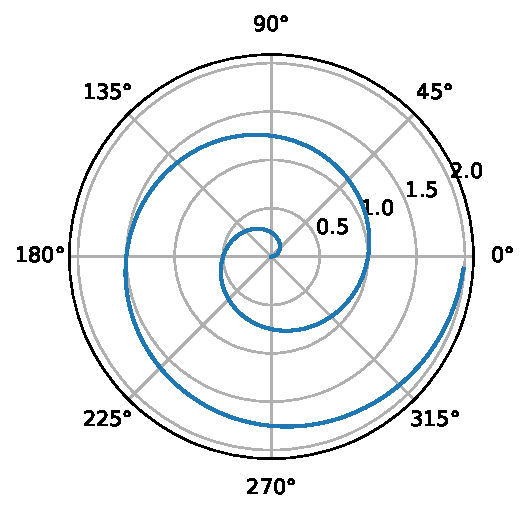
\includegraphics[keepaspectratio]{cOSX_files/figure-latex/fig-polar-output-1.pdf}}

}

\caption{\label{fig-polar}A line plot on a polar axis}

\end{figure}%

And the command was \texttt{quarto\ render\ test.qmd\ -\/-to\ html}.

And if you \texttt{brew\ install\ texlive} then export to pdf works well
too.

\chapter{Python}\label{python-1}

\chapter{Virtual Environments}\label{virtual-environments}

The advantage of a virtual environment is the ability to isolate
libraries you may install for a particular project from interfering with
other projects or previously installed libraries. The disadvantage is
that they do involve some additional steps and complexity and you may
end up installing multiple versions of the same library, which can be an
issue if hard disk space on your computer is limited.

\section{Methods}\label{methods}

There is more than one tool for creating a python virutal environment,
but one of them is built into the standard python installation:
\emph{venv}, and so for simplicity this is the one that I recommend
starting with.

\subsection{Creating and Activating the
Venv}\label{creating-and-activating-the-venv}

If you are in a console you can simply run these commands in the
terminal.

\begin{Shaded}
\begin{Highlighting}[]
\NormalTok{python {-}m venv \textless{}dir{-}where{-}you{-}want{-}venv\textgreater{}}
\NormalTok{cd \textless{}dir{-}where{-}you{-}want{-}venv\textgreater{}}
\NormalTok{source ./bin/activate}
\end{Highlighting}
\end{Shaded}

\begin{tcolorbox}[enhanced jigsaw, opacityback=0, leftrule=.75mm, colback=white, left=2mm, titlerule=0mm, toprule=.15mm, toptitle=1mm, coltitle=black, title=\textcolor{quarto-callout-note-color}{\faInfo}\hspace{0.5em}{Note}, opacitybacktitle=0.6, colbacktitle=quarto-callout-note-color!10!white, breakable, bottomrule=.15mm, bottomtitle=1mm, colframe=quarto-callout-note-color-frame, arc=.35mm, rightrule=.15mm]

Depending on the specifics of your operating system and python
installation you may find you need to use \texttt{python3} and
\texttt{pip3} commands instead of plain \texttt{python} and
\texttt{pip}.

\end{tcolorbox}

If you are using a Windows device you will have to find your equivalent
of a linux terminal. This can be using
\href{https://learn.microsoft.com/en-us/windows/wsl/install}{WSL} or
something like \href{https://en.wikipedia.org/wiki/MinGW}{MinGW}.

Once you have activated your \texttt{venv} you will see a change in the
terminal display that indicates the \texttt{venv} is active. Now when
you run things like
\texttt{pip\ install\ \textless{}something\textgreater{}} it will
install that library to a sandbox that is only accessible when using
python from within that virtual environment. You should note that this
notion of a sandbox or virtual environment is also available for some
other programming languages.

To deactivate the environment you run ,

\begin{Shaded}
\begin{Highlighting}[]
\NormalTok{deactivate}
\end{Highlighting}
\end{Shaded}

from within the venv. Look for the change in the terminal display. Note
how activating the environment shows up in the terminal prompt.

\begin{Shaded}
\begin{Highlighting}[]
\NormalTok{britt@arts{-}220486 \textasciitilde{} \% source p390venv/bin/activate}
\NormalTok{(p390venv) britt@arts{-}220486 \textasciitilde{} \% deactivate}
\NormalTok{britt@arts{-}220486 \textasciitilde{} \% }
\end{Highlighting}
\end{Shaded}

\subsection{The Terminal is All You
Need}\label{the-terminal-is-all-you-need}

If you are a minimalist or doing something simple you can invoke the
python interpreter in your venv and complete your task there with no
other tools, and using only the libraries required for your particular,
limited task. However, if you use some companion tooling things may get
more complicated and trickier to debug.

\section{Visual Studio Code}\label{visual-studio-code}

VS Code tries to make using a venv easier, but this also means there is
some indirection that may make it harder to puzzle out errors. The basic
work flow is to make sure that VS code is working in the folder you want
your venv to be in. If not, use the \texttt{open\ folder} menu of VS
Code to do so. Then, you can use the \texttt{Command\ Palette} (found
under the \emph{View} menu tab) to locate the
\texttt{Python\ Create\ Environment} command. If you have never created
an environment before it will do so. This can take some time so be
patient and make sure this process completes. If there was a virtual
environment previously constructed VS Code will probably be able to
figure that out and ask you if you want to re-use it. Usually you will,
but if not you can select to destroy it and create a new one. You will
probably also need to affilate a particular python version to
association to your environment. VS Code can often make a reasonable
suggestion and you can also use the command
\texttt{Python\ Select\ Interpreter} if necessary.

After you have done that you will need to move into the affiliated
terminal window of your VS Code environment to install the necessary
libraries. You will need to be deliberate and make sure that you are in
the correct terminal. VS Code may have several of these open for
different purposes if you are working on a complicated project.

Note that while it may be convenient to use the VS Code terminals you do
not have to. If you have a terminal program on your computer accessible
to you outside of VS Code you can use VS Code as the editor and then
move to your other terminal for activating and implementing and
compiling the python project.

\subsection{Quarto Complications}\label{quarto-complications}

When you embed a python code block in your .qmd document you will want
to compile it. Quarto is assembling a document. It will need more than
just the libraries necessary for compiling the python code. It also
needs the library for the textual and graphical representation of the
output that you will insert into your document. Specifically, it needs
the \texttt{jupyter} python library. This means that whatever the python
is doing, even if no additional libraries are needed, you will have to
have done a \texttt{pip\ install\ jupyter} in your venv \emph{and} you
will need to have the venv active for the location where the qmd is
stored and compiled.

It is worth knowing that although VS Code offers the convenience of
buttons to invoke the quarto process it is \emph{not} necessary. You can
invoke all the quarto commands through a terminal directly. For instance
\texttt{quarto\ preview\ \textless{}file-name\textgreater{}.qmd} will
try to compile your file and will also usually launch your browser so
you can see the html result. It will then watch the source file and
update the html whenever it detects you have changed the source. This
can be quite convenient for editing.

\phantomsection\label{refs}
\begin{CSLReferences}{1}{0}
\bibitem[\citeproctext]{ref-Duan_2024}
Duan, Xufeng, Shixuan Li, and Zhenguang G. Cai. 2024. {``MacBehaviour:
An r Package for Behavioural Experimentation on Large Language
Models.''} \emph{Behavior Research Methods} 57 (1).
\url{https://doi.org/10.3758/s13428-024-02524-y}.

\end{CSLReferences}




\end{document}
